%─────Lecture 3──────────────────────────────────────────────────────────────────────────────────────────────────────────────────────────────────────
\chapter{Option Basics}
\label{ch:option-basics}
\marginpar{\footnotesize\textsf{\raggedright Lecture 3\\ September 24, 2026}}

% ── Black–Scholes helpers for the value/profit pictures in this chapter ──
% pgfmath has no erf, so the standard normal CDF is the Abramowitz–Stegun
% 26.2.17 rational approximation (absolute error < 7.5e-8).
\pgfmathdeclarefunction{nphi}{1}{\pgfmathparse{exp(-0.5*(#1)^2)/sqrt(2*pi)}}
\pgfmathdeclarefunction{nt}{1}{\pgfmathparse{1/(1+0.2316419*abs(#1))}}
\pgfmathdeclarefunction{ntail}{1}{\pgfmathparse{nphi(#1)*nt(#1)*(0.319381530+nt(#1)*(-0.356563782+nt(#1)*(1.781477937+nt(#1)*(-1.821255978+nt(#1)*1.330274429))))}}
\pgfmathdeclarefunction{ncdf}{1}{\pgfmathparse{ifthenelse(#1>0,1-ntail(#1),ntail(#1))}}
% Parameters used throughout: r = 5%, sigma = 30%, tau = 1 month.
%   sigma*sqrt(tau) = 0.0866025, (r+sigma^2/2)*tau = 0.0079167, e^{-r tau} = 0.9958420.
\pgfmathdeclarefunction{bsdone}{2}{\pgfmathparse{(ln((#1)/(#2))+0.0079167)/0.0866025}}
\pgfmathdeclarefunction{bscall}{2}{\pgfmathparse{(#1)*ncdf(bsdone(#1,#2))-(#2)*0.9958420*ncdf(bsdone(#1,#2)-0.0866025)}}
\pgfmathdeclarefunction{bsput}{2}{\pgfmathparse{bscall(#1,#2)-(#1)+(#2)*0.9958420}}

\source{Slides pp.~185--186}

\begin{flushright}
	\itshape The shift toward options as\\
	the center of gravity of finance [\ldots]\\
	\upshape --- Merton H.~Miller\footnote{Co-winner of the 1990 Nobel Prize in Economic Sciences.} (1923--2000)

	\medskip

	\itshape Too many potential physicists and engineers\\
	spend their careers shifting money around\\
	in the financial sector,\\
	instead of applying their talents to\\
	innovating in the real economy.\\
	\upshape --- Barack Obama (2016)
\end{flushright}

\bigskip

\noindent Every instrument so far has had a cash flow that is \emph{fixed} the moment the contract is signed.
A bond pays its coupons whether the world turns out well or badly; the only uncertainty is the rate at which we discount them, and all of Chapters~3 and~4 was about that rate.
An option is the first instrument in this course whose cash flow at expiration is \vocab{contingent}: it depends on what the underlying asset happens to be worth on that day.

That single change is what makes the pricing problem hard, and it is the problem the rest of the course solves.
This chapter, however, prices nothing.
Its job is to fix
\begin{enumerate}[(i)]
	\item the vocabulary --- call, put, strike, exercise, American, European;
	\item the \emph{payoff functions}, which are the terminal conditions every later pricing model must reproduce;
	\item the market conventions that decide what the contract actually promises --- dividends, splits, short selling; and
	\item the standard portfolios built out of options: hedges, spreads, and combinations.
\end{enumerate}
The last item is worth more than it looks.
Two of the spreads below, pushed to a limit, deliver model-\emph{independent} prices for two exotic securities, and --- pushed one step further --- read the market's own probability distribution for $S_{T}$ straight off the quoted call prices.
All of that comes for free, before writing down any stochastic process at all.

%─────§1 Calls and puts──────────────────────────────────────────────────────────────────────────────────────────────────────────────────────────────
\section{Calls and Puts}
\label{sec:calls-puts}

\source{Slides pp.~187--189}

\begin{definition}
	A \vocab{call} gives its holder the \emph{right}, but not the obligation, to \emph{buy} one unit of the underlying asset by paying a \vocab{strike price} (also called the exercise price).
\end{definition}

The holder pays for that right up front.
The price paid is the \vocab{option premium}, and it is the only cash flow that is certain: the cash flow at expiration is contingent, because the holder will simply walk away if buying at the strike is a bad deal.
\autoref{fig:call-cashflow} draws the two dates.

\begin{figure}[H]
	\centering
	\begin{tikzpicture}[font=\small, >={Stealth[length=5pt]}]
		\draw[->] (-0.4,0) -- (9.0,0) node[right] {time};
		% premium paid today
		\draw[->, RawSienna, thick] (1.0,0) -- (1.0,-1.0);
		\node[below, RawSienna] at (1.0,-1.05) {option premium};
		\node[above=1pt, font=\footnotesize, text=Gray!60!black] at (1.0,0) {today};
		% expiration
		\draw[->, MidnightBlue!75!black, thick] (6.4,0) -- (6.4,1.35);
		\node[above, MidnightBlue!75!black] at (6.4,1.4) {stock};
		\draw[->, RawSienna, thick] (6.4,0) -- (6.4,-1.0);
		\node[below, RawSienna] at (6.4,-1.05) {strike price};
		\node[anchor=south west, font=\footnotesize, text=Gray!60!black]
		at (6.55,0.05) {expiration};
	\end{tikzpicture}
	\caption{Cash flows of a long call. Arrows below the axis are payments made
		by the holder, arrows above it are receipts. The premium leaves today
		with certainty; the exchange of the strike price for the stock happens
		at expiration \emph{only if} the holder chooses to exercise.}
	\label{fig:call-cashflow}
\end{figure}

\begin{definition}
	A \vocab{put} gives its holder the right to \emph{sell} one unit of the underlying asset for the strike price.
\end{definition}

The put reverses the two contingent arrows: the holder delivers the stock and receives the strike price (\autoref{fig:put-cashflow}).
The premium still leaves today.

\begin{figure}[H]
	\centering
	\begin{tikzpicture}[font=\small, >={Stealth[length=5pt]}]
		\draw[->] (-0.4,0) -- (9.0,0) node[right] {time};
		\draw[->, RawSienna, thick] (1.0,0) -- (1.0,-1.0);
		\node[below, RawSienna] at (1.0,-1.05) {option premium};
		\node[above=1pt, font=\footnotesize, text=Gray!60!black] at (1.0,0) {today};
		\draw[->, MidnightBlue!75!black, thick] (6.4,0) -- (6.4,1.35);
		\node[above, MidnightBlue!75!black] at (6.4,1.4) {strike price};
		\draw[->, RawSienna, thick] (6.4,0) -- (6.4,-1.0);
		\node[below, RawSienna] at (6.4,-1.05) {stock};
		\node[anchor=south west, font=\footnotesize, text=Gray!60!black]
		at (6.55,0.05) {expiration};
	\end{tikzpicture}
	\caption{Cash flows of a long put --- \autoref{fig:call-cashflow} with the
		roles of stock and strike price interchanged.}
	\label{fig:put-cashflow}
\end{figure}

\begin{notation}
	Options sold on their own, as the two figures above assume, are called \emph{standalone}.
	An \vocab{embedded option} is one that cannot be separated from its host: it has to be traded along with the underlying asset.
	The callable bond of Chapter~3 is the standing example --- the issuer's right to redeem early is an option, but nobody trades it apart from the bond.
\end{notation}

\begin{remark}
	How to price options?
	That is the question the next several chapters answer, and it is old: it can be traced to Aristotle's (384 B.C.--322 B.C.) \emph{Politics}, if not earlier.\footnote{Aristotle reports that Thales, foreseeing a large olive harvest, paid deposits in winter for the use of every olive press in Miletus and Chios --- the deposits are option premiums, and the presses are the underlying asset.}
\end{remark}

%─────§2 Exercise────────────────────────────────────────────────────────────────────────────────────────────────────────────────────────────────────
\section{Exercise}

\source{Slides p.~190}

To \vocab{exercise} an option is to invoke the right it grants, and the mechanics are exactly the two contingent arrows drawn above:

\begin{itemize}[itemsep=0.3em]
	\item When a \emph{call} is exercised, the holder pays the strike price in exchange for the stock.
	\item When a \emph{put} is exercised, the holder receives the strike price from the writer in exchange for the stock.
\end{itemize}

\noindent The counterparty --- the \vocab{writer}, who sold the option and pocketed the premium --- has no choice in the matter: the writer must take the other side whenever the holder exercises.
This asymmetry is the whole content of the word ``option''.

Some options may be exercised \emph{before} the expiration date.
This is called \vocab{early exercise}, and deciding whether to do it is an optimization problem in its own right, not a detail of the contract.
\autoref{sec:early-exercise} settles the question completely for calls; for puts it stays open for the rest of the course.

%─────§3 American and European───────────────────────────────────────────────────────────────────────────────────────────────────────────────────────
\section{American and European}

\source{Slides p.~191}

\begin{definition}
	An \vocab{American option} can be exercised at any time up to the expiration date.
	A \vocab{European option} can only be exercised at expiration.
\end{definition}

\begin{proposition}
	\label{prop:amer-ge-euro}
	An American option is worth at least as much as an otherwise identical European option.
\end{proposition}

\begin{proof}
	The American contract contains every right the European contract contains, plus the right to exercise early.
	The holder of the American option may simply choose never to exercise early, thereby reproducing the European payoff exactly.
	A strictly larger set of available strategies cannot be worth less.
\end{proof}

\begin{note}
	The names are geographical only by accident; both types trade on both continents.
	Note also that \autoref{prop:amer-ge-euro} is an inequality, not an equality --- and the gap is genuinely hard to compute.
	European options on a non-dividend-paying stock admit a closed-form price (Black--Scholes); American puts do not, which is why so much of the numerical machinery later in the course exists --- \autoref{sec:early-exercise} proves the gap is \emph{zero} for calls on such a stock, and \autoref{sec:american-one-period} shows where it reopens for puts.
\end{note}

%─────§4 Conventions─────────────────────────────────────────────────────────────────────────────────────────────────────────────────────────────────
\section{Convenient Conventions}

\source{Slides p.~192}

\begin{notation}
	The following symbols are used without further comment for the rest of the course.
	\begin{center}
		\begin{tabular}{@{}cl@{}}
			\toprule
			Symbol & Meaning              \\
			\midrule
			$C$    & call value           \\
			$P$    & put value            \\
			$X$    & strike price         \\
			$S$    & stock price          \\
			$D$    & dividend             \\
			\bottomrule
		\end{tabular}
	\end{center}
	We always assume $S\ge 0$.\footnote{Contributed by Mr.~Tang, Bert (B08902102) on March 10, 2021.}
	When the time matters we write $S_{t}$ for the stock price at time $t$, and $S_{T}$ for its value at expiration.
\end{notation}

%─────§5 Payoffs────────────────────────────────────────────────────────────────────────────────────────────────────────────────────────────────────
\section{Payoff, Mathematically Speaking}
\label{sec:payoff}

\source{Slides pp.~193--194}

At expiration the holder's decision is trivial, because there is no future left to speculate about: exercise if and only if doing so produces cash.

\begin{definition}
	The \vocab{payoff} of a call at expiration is
	\begin{equation}
		C \;=\; \max(0,\, S-X) ,
		\label{eq:call-payoff}
	\end{equation}
	and the payoff of a put at expiration is
	\begin{equation}
		P \;=\; \max(0,\, X-S) .
		\label{eq:put-payoff}
	\end{equation}
\end{definition}

The $\max(0,\cdot)$ is the contract's optionality made arithmetic.
A call will be exercised only if the stock price is \emph{higher} than the strike price --- otherwise the stock can be bought more cheaply in the market, and the holder lets the option lapse.
Symmetrically, a put will be exercised only if the stock price is \emph{less} than the strike price.

\begin{moral}
	Two facts about \eqref{eq:call-payoff} and \eqref{eq:put-payoff} drive everything that follows.

	They are \emph{non-negative}: an option can never impose a loss on its holder beyond the premium already paid.
	Hence $C\ge 0$ and $P\ge 0$ at \emph{all} times, not just at expiration.

	They are \emph{convex} and \emph{kinked} at $S=X$.
	Convexity is why options are worth more than their intrinsic value before expiration (Jensen's inequality again), and the kink is the single point where every numerical method in this course has to work hardest.
\end{moral}

\autoref{fig:payoff-four} draws all four elementary positions with $X=50$.
The writer's payoff is the holder's payoff reflected through the horizontal axis --- options are a zero-sum contract between the two parties, so the two pictures in each column must sum to zero pointwise.

\begin{figure}[htbp]
	\centering
	\begin{tikzpicture}[font=\footnotesize]
		\begin{groupplot}[
				group style={group size=2 by 2, horizontal sep=1.9cm,
						vertical sep=1.55cm},
				width=0.46\textwidth, height=4.3cm,
				xmin=0, xmax=92, xtick={20,40,60,80},
				axis lines=middle,
				axis line style={-{Stealth[length=4pt]}, thin},
				tick label style={font=\scriptsize},
				title style={font=\small, text=Gray!40!black},
				xlabel={Price}, ylabel={Payoff},
				every axis x label/.style={at={(ticklabel cs:1.0)}, anchor=west},
				every axis y label/.style={at={(ticklabel cs:1.0)}, rotate=0,
						anchor=south},
				every axis plot post/.append style={MidnightBlue!80!black,
						very thick, mark=none},
				clip=false,
			]
			\nextgroupplot[title={Long a call}, ymin=0, ymax=42, ytick={10,20,30,40}]
			\addplot coordinates {(0,0) (50,0) (90,40)};

			\nextgroupplot[title={Short a call}, ymin=-42, ymax=0, xticklabel style={anchor=south, yshift=2pt}, title style={yshift=10pt},
				ytick={-40,-30,-20,-10}]
			\addplot coordinates {(0,0) (50,0) (90,-40)};

			\nextgroupplot[title={Long a put}, ymin=0, ymax=52, ytick={10,20,30,40,50}]
			\addplot coordinates {(0,50) (50,0) (90,0)};

			\nextgroupplot[title={Short a put}, ymin=-52, ymax=0, xticklabel style={anchor=south, yshift=2pt}, title style={yshift=10pt},
				ytick={-50,-40,-30,-20,-10}]
			\addplot coordinates {(0,-50) (50,0) (90,0)};
		\end{groupplot}
	\end{tikzpicture}
	\caption{Payoffs at expiration of the four elementary option positions,
		with strike $X=50$. These are payoffs, not profits: the premium has
		not been subtracted. The kink always sits at $S=X$. Note the
		asymmetry in the writer's risk --- a short call has unbounded loss as
		$S\to\infty$, whereas a short put loses at most $X$, since the stock
		cannot fall below zero.}
	\label{fig:payoff-four}
\end{figure}

\subsection{Intrinsic Value and Moneyness}

\source{Slides pp.~195--196}

\begin{definition}
	At any time $t$ \emph{before} the expiration date, the \vocab{intrinsic value} of a call is
	\[
		\max(0,\, S_{t}-X) ,
	\]
	and the intrinsic value of a put is
	\[
		\max(0,\, X-S_{t}) .
	\]
\end{definition}

The intrinsic value is what the option would pay if expiration were today.
It is a \emph{lower} bound on an American option's value (exercising is always available) and, as \autoref{lem:call-intrinsic} will show, a lower bound on a European \emph{call}'s value as well --- though not, it turns out, on a European put's.
Whatever the option is worth above its intrinsic value is its \vocab{time value} --- the market's charge for the remaining chance that the stock moves further in the holder's favour.

\begin{definition}
	A call is \vocab{in the money} if $S>X$, \vocab{at the money} if $S=X$, and \vocab{out of the money} if $S<X$.
	A put is in the money if $S<X$, at the money if $S=X$, and out of the money if $S>X$.
\end{definition}

\begin{note}
	The direction reverses between calls and puts, so the words describe \emph{whether the option currently has positive intrinsic value}, not whether the stock is high or low.
\end{note}

Options that are in the money at expiration should be exercised --- the payoff is positive and free.
Astonishingly, they are not always.\footnote{About 11\% of option holders let in-the-money options expire worthless.}

Finding an option's value at \emph{any} time before expiration --- that is, splitting it into intrinsic value plus time value with an actual number attached --- is a major intellectual breakthrough. Chapter~\ref{ch:pricing-models} makes it, and the rest of the course elaborates on it.

\source{Slides p.~197}

\autoref{fig:option-value} shows what the answer looks like ahead of time.
The dashed line in each panel is the intrinsic value, the payoff already drawn in \autoref{fig:payoff-four}; the solid curve is the option's value one month before expiration.
Three features are visible and will be proved later:

\begin{itemize}[itemsep=0.3em]
	\item The solid curve is \emph{smooth}: the kink at $S=X$ has been rounded off, because with time left the market does not yet know which side of the strike the stock will land on.
	\item The call's curve lies \emph{above} its intrinsic value everywhere --- that gap is time value --- and is monotone and convex, sandwiched between the intrinsic value and the stock price itself.
	\item The put's curve does \emph{not}. Look at the left edge of the right-hand panel: for small $S$ the solid curve dips \emph{below} the dashed one, so a European put can be worth less than its intrinsic value. This is not a drawing error, and \autoref{lem:put-bound} explains it.
\end{itemize}

\begin{figure}[H]
	\centering
	\begin{tikzpicture}[font=\footnotesize]
		\begin{groupplot}[
				group style={group size=2 by 1, horizontal sep=1.6cm},
				width=0.47\textwidth, height=4.8cm,
				xmin=80, xmax=115, xtick={80,85,90,95,100,105,110,115},
				ymin=0,
				xlabel={Stock price},
				title style={font=\small, text=Gray!40!black},
				tick label style={font=\scriptsize},
				label style={font=\scriptsize},
				axis line style={thin}, tick align=outside,
				clip=false,
			]
			\nextgroupplot[title={Call value}, ymax=21.5, ytick={0,5,10,15,20}]
			\addplot[Gray!55!black, densely dashed, thick]
			coordinates {(80,0) (95,0) (115,20)};
			\addplot[MidnightBlue!80!black, very thick, domain=80:115,
				samples=120] {bscall(x,95)};

			\nextgroupplot[title={Put value}, ymax=15.5, ytick={0,2,4,6,8,10,12,14}]
			\addplot[Gray!55!black, densely dashed, thick]
			coordinates {(80,15) (95,0) (115,0)};
			\addplot[RawSienna, very thick, domain=80:115, samples=120]
			{bsput(x,95)};
		\end{groupplot}
	\end{tikzpicture}
	\caption{Value of a European call and put with strike $X=95$ one month
		before expiration (solid), against their intrinsic values (dashed).
		Computed from Black--Scholes with $r=5\%$ and $\sigma=30\%$; the
		formula itself is derived much later, and only the \emph{shape}
		matters here. The vertical gap between the two lines is the time
		value, largest at the money and vanishing deep in or out of the
		money.}
	\label{fig:option-value}
\end{figure}

%─────§6 Dividends and splits────────────────────────────────────────────────────────────────────────────────────────────────────────────────────────
\section{Corporate Actions: Dividends and Splits}
\label{sec:corporate-actions}

The payoff formulas above refer to ``the stock'', but a share is not a fixed object: companies pay dividends and split their shares, and each event moves $S$ for reasons that have nothing to do with the market's opinion of the company.
Whether the option contract is \emph{adjusted} for such an event therefore changes what the option is worth.
The convention differs by event type.

\subsection{Cash Dividends}

\source{Slides p.~198}

Exchange-traded stock options are \emph{not} cash dividend-protected (or simply \vocab{protected}): the option contract is not adjusted for cash dividends.

Why this matters: on the \vocab{ex-dividend} date the stock price falls by an amount roughly equal to the cash dividend, because a buyer from that day on no longer receives it.
The drop is mechanical, but the unprotected option absorbs it in full.
Consequently

\begin{center}
	\emph{cash dividends are detrimental for calls, and the opposite is true for puts.}
\end{center}

\begin{intuition}
	The option holder owns exposure to the share price but not the share, and therefore collects no dividend.
	A dividend transfers value out of the share price and into the pockets of shareholders --- over whom the call holder has no claim.
	So a call on a dividend-paying stock is worth less than a call on an otherwise identical stock that retains its cash, and a put is worth correspondingly more.
	This is also the reason early exercise of an American call can be optimal: exercising just before the ex-dividend date is the only way to capture the dividend. \autoref{thm:merton-dividend} makes that precise --- those dates are the \emph{only} ones at which it can pay to exercise early.
\end{intuition}

\subsection{Stock Splits and Stock Dividends}

\source{Slides pp.~199--200}

Options \emph{are} adjusted for stock splits.
After an \vocab{$n$-for-$m$ stock split}, $m$ shares become $n$ shares.
Accordingly, the option is rewritten so that

\begin{itemize}[nosep]
	\item the strike price becomes $m/n$ times its previous value, and
	\item the number of shares covered by one option becomes $n/m$ times its previous value.
\end{itemize}

\noindent Exchange-traded stock options are adjusted for \vocab{stock dividends} in the same way.
The point of the adjustment is that the total strike outlay $X\times(\text{shares covered})$ is unchanged, so the split --- which alters nothing real about the company --- alters nothing about the option.

\begin{eg}
	Consider an option to buy 100 shares of a company for \$50 per share.
	A 2-for-1 split changes the terms to a strike price of \$25 per share for 200 shares.
	The outlay on exercise is $100\times 50 = 200\times 25 = \$5{,}000$ either way.
\end{eg}

\begin{note}
	Unless stated otherwise, \textbf{we assume options are unprotected} from here on.
	Cash dividends will therefore show up explicitly as a term in every pricing formula, while splits will never be mentioned again.
\end{note}

%─────§7 Short selling───────────────────────────────────────────────────────────────────────────────────────────────────────────────────────────────
\section{Short Selling}
\label{sec:short-selling}

\source{Slides pp.~201--203}

Several of the portfolios below, and essentially every no-arbitrage argument later in the course, require taking a \emph{negative} position in the stock. The mechanism that makes this possible is short selling.

\begin{definition}
	\vocab{Short selling} (or \vocab{shorting})\footnote{Invented by Le Maire (1558--1624) in 1608.} means selling an asset that is not owned, with the intention of buying it back later.
\end{definition}

Concretely, if you short 1{,}000 XYZ shares:

\begin{enumerate}[itemsep=0.25em]
	\item The broker borrows the 1{,}000 shares from another client and sells them in the market.
	\item This action generates proceeds for the investor --- cash now, and an obligation to return the shares later.
	\item The investor closes out the short position by buying 1{,}000 XYZ shares and returning them.
\end{enumerate}

\noindent Clearly, the investor profits if the stock price falls: the repurchase costs less than the sale brought in.
The payoff of a short position is the payoff of a long position with the sign flipped (\autoref{fig:stock-payoff}), which is exactly the property that makes shorting the algebraic tool it is.

\begin{figure}[H]
	\centering
	\begin{tikzpicture}[font=\footnotesize]
		\begin{groupplot}[
				group style={group size=2 by 1, horizontal sep=1.9cm},
				width=0.46\textwidth, height=4.3cm,
				xmin=0, xmax=92, xtick={20,40,60,80},
				axis lines=middle,
				axis line style={-{Stealth[length=4pt]}, thin},
				tick label style={font=\scriptsize},
				title style={font=\small, text=Gray!40!black},
				xlabel={Price}, ylabel={Payoff},
				every axis x label/.style={at={(ticklabel cs:1.0)}, anchor=west},
				every axis y label/.style={at={(ticklabel cs:1.0)}, rotate=0,
						anchor=south},
				every axis plot post/.append style={MidnightBlue!80!black,
						very thick, mark=none},
				clip=false,
			]
			\nextgroupplot[title={Long a stock}, ymin=0, ymax=92,
				ytick={20,40,60,80}]
			\addplot coordinates {(0,0) (90,90)};

			\nextgroupplot[title={Short a stock}, ymin=-92, ymax=0, xticklabel style={anchor=south, yshift=2pt}, title style={yshift=10pt},
				ytick={-80,-60,-40,-20}]
			\addplot coordinates {(0,0) (90,-90)};
		\end{groupplot}
	\end{tikzpicture}
	\caption{Payoff of a stock position. Unlike the option payoffs of
		\autoref{fig:payoff-four} these are straight lines through the
		origin --- the stock has no kink, and hence no optionality.}
	\label{fig:stock-payoff}
\end{figure}

\begin{note}
	Two warnings, both of which the models we build will quietly ignore.

	Not all assets can be shorted --- there must be a lender, and lendable inventory is neither free nor guaranteed.

	In reality, short selling is not simply the opposite of going long.\footnote{Kosowski \& Neftci (2015). See \url{https://tw.news.appledaily.com/headline/daily/20180307/37950481/} for an example in Taiwan on February 6, 2018.}
	The short seller pays a borrowing fee, can be forced to close the position when the lender recalls the shares, faces an unbounded loss, and may be barred from shorting altogether by regulators in a falling market.
\end{note}

%─────§8 Covered positions: hedges───────────────────────────────────────────────────────────────────────────────────────────────────────────────────
\section{Covered Positions: Hedges}
\label{sec:hedges}

\source{Slides pp.~204--205}

A \vocab{covered position} is an option combined with other securities.
Three families are worth naming: \emph{hedges}, which combine an option with its own underlying stock; \emph{spreads} (\autoref{sec:option-spreads}), which combine options of the \emph{same} type; and \emph{combinations} (\autoref{sec:combinations}), which mix calls with puts.

\begin{definition}
	A \vocab{hedge} combines an option with its underlying stock in such a way that one protects the other against loss.
\end{definition}

\noindent Two hedges account for almost all practical use:

\begin{itemize}[itemsep=0.35em]
	\item \vocab{Covered call}: a long position in the stock together with a \emph{short} call.\footnote{A short position has a payoff opposite in sign to that of a long position, as in \autoref{fig:payoff-four}. Some ETFs package this payoff directly, such as the Global X Nasdaq 100 Covered Call ETF (QYLD).}
	      It is called ``covered'' because the stock on hand can be delivered to the buyer of the call if the call is exercised --- the writer is never forced to buy at an arbitrarily high market price.

	\item \vocab{Protective put}: a long position in the stock together with a \emph{long} put.
	      The put is an insurance policy on the shares: whatever happens, they can be sold for at least $X$.
\end{itemize}

Writing $S_{T}$ for the stock price at expiration, the two payoffs are
\begin{equation}
	\begin{aligned}
		\text{covered call:}\quad   & S_{T}-\max(0,S_{T}-X) \;=\; \min(S_{T},\,X) , \\
		\text{protective put:}\quad & S_{T}+\max(0,X-S_{T}) \;=\; \max(S_{T},\,X) .
	\end{aligned}
	\label{eq:hedge-payoffs}
\end{equation}
So the covered call \emph{caps} the outcome at $X$ and the protective put \emph{floors} it at $X$.

\begin{note}
	Both strategies break even only if the stock price rises above a certain level, so \textbf{both are bullish}.
	This is easy to miss, because a covered call is often described as ``defensive''.
	The premium received merely offsets a fixed amount of downside; the position still loses roughly dollar-for-dollar with the stock once that cushion is gone, as the left-hand tail in \autoref{fig:hedge-profit} shows.
\end{note}

\begin{figure}[H]
	\centering
	\begin{tikzpicture}[font=\footnotesize]
		\begin{groupplot}[
				group style={group size=2 by 1, horizontal sep=1.8cm},
				width=0.47\textwidth, height=4.8cm,
				xmin=81, xmax=111, xtick={85,90,95,100,105,110},
				axis lines=middle,
				axis line style={-{Stealth[length=4pt]}, thin},
				tick label style={font=\scriptsize},
				title style={font=\small, text=Gray!40!black},
				xlabel={Stock price}, ylabel={Profit},
				every axis x label/.style={at={(ticklabel cs:1.0)}, anchor=north east,
						yshift=-7pt},
				every axis y label/.style={at={(ticklabel cs:1.0)}, rotate=0,
						anchor=south},
				clip=false,
			]
			\nextgroupplot[title={Protective put}, ymin=-4.5, ymax=13,
				ytick={-2.5,2.5,5,7.5,10,12.5},
				yticklabel style={/pgf/number format/fixed}]
			\addplot[Gray!55!black, densely dashed, thick]
			coordinates {(81,-3.081) (95,-3.081) (110,11.919)};
			\addplot[MidnightBlue!80!black, very thick, domain=81:110,
				samples=110] {x+bsput(x,95)-95-3.081};

			\nextgroupplot[title={Covered call}, ymin=-13, ymax=4,
				ytick={-12,-10,-8,-6,-4,-2,2}]
			\addplot[Gray!55!black, densely dashed, thick]
			coordinates {(81,-10.526) (95,3.476) (110,3.476)};
			\addplot[RawSienna, very thick, domain=81:110, samples=110]
			{x-bscall(x,95)-95+3.476};
		\end{groupplot}
	\end{tikzpicture}
	\caption{Profit of the two hedges, with $X=95$ and the portfolio set up
		when $S=95$ one month before maturity. Dashed lines are profits at
		expiration, given by \eqref{eq:hedge-payoffs} less the setup cost.
		Solid lines are profits at the moment the portfolio is set up, as a
		function of where the stock price goes; they are smooth because the
		options still carry time value. Both pictures slope upward on the
		left, which is what ``bullish'' means.}
	\label{fig:hedge-profit}
\end{figure}

%─────§9 Covered positions: spreads──────────────────────────────────────────────────────────────────────────────────────────────────────────────────
\section{Covered Positions: Spreads}
\label{sec:option-spreads}

\source{Slides p.~206}

\begin{definition}
	A \vocab{spread} consists of options of the same type and on the same underlying asset, but with different strike prices or expiration dates.
\end{definition}

Throughout this section we use $X_{L}$, $X_{M}$, and $X_{H}$ to denote strike prices with
\[
	X_{L} \;<\; X_{M} \;<\; X_{H} .
\]
All options in a spread are calls, or all are puts; mixing types produces a \emph{combination} instead, which is \autoref{sec:combinations}.

\subsection{Bull Spreads}

\source{Slides pp.~207--208}

\begin{definition}
	A \vocab{bull call spread} consists of a long $X_{L}$ call and a short $X_{H}$ call with the same expiration date.
\end{definition}

Since $C_{L}>C_{H}$ (a lower strike is worth more), the position costs money to enter.
Its accounting is completely determined by \eqref{eq:call-payoff}:

\begin{itemize}[itemsep=0.3em]
	\item The initial investment is $C_{L}-C_{H}$.
	\item The payoff is nonnegative; explicitly it is $\max(0,S_{T}-X_{L})-\max(0,S_{T}-X_{H})$.
	\item The maximum payoff is $X_{H}-X_{L}$, achieved when both calls are exercised at expiration, i.e.\ when $S_{T}\ge X_{H}$.
	\item The maximum profit is therefore $(X_{H}-X_{L})-(C_{L}-C_{H})$.
	\item The maximum loss is $C_{L}-C_{H}$, incurred when neither is exercised at expiration, i.e.\ when $S_{T}\le X_{L}$.
\end{itemize}

\noindent Both the gain and the loss are bounded: the short call pays for part of the long call and, in exchange, sells away every gain above $X_{H}$.
The investor is betting that the stock rises, but only so far.

\begin{figure}[H]
	\centering
	\begin{tikzpicture}[font=\footnotesize]
		\begin{axis}[
				width=0.72\textwidth, height=5.2cm,
				xmin=81, xmax=111, xtick={85,90,95,100,105,110},
				ymin=-6, ymax=6, ytick={-4,-2,2,4},
				axis lines=middle,
				axis line style={-{Stealth[length=4pt]}, thin},
				tick label style={font=\scriptsize},
				title style={font=\small, text=Gray!40!black},
				title={Bull spread (call)},
				xlabel={Stock price}, ylabel={Profit},
				every axis x label/.style={at={(ticklabel cs:1.0)}, anchor=west},
				every axis y label/.style={at={(ticklabel cs:1.0)}, rotate=0,
						anchor=south},
				clip=false,
			]
			\addplot[Gray!55!black, densely dashed, thick]
			coordinates {(81,-5.016) (90,-5.016) (100,4.984) (111,4.984)};
			\addplot[MidnightBlue!80!black, very thick, domain=81:110,
				samples=120] {bscall(x,90)-bscall(x,100)-5.016};
		\end{axis}
	\end{tikzpicture}
	\caption{Profit of a bull call spread with $X_{L}=90$, $X_{H}=100$,
		entered when $S=95$ one month before expiration for a net debit of
		$C_{L}-C_{H}=5.02$. Dashed: profit at expiration, a ramp clipped at
		both ends. Solid: profit at the moment of entry as the stock price
		varies. The maximum profit $4.98$ and the maximum loss $5.02$ are the
		two dashed plateaus.}
	\label{fig:bull-spread}
\end{figure}

\subsection{The Binary Call: A Model-Free Price}
\label{sec:binary-call}

\source{Slides p.~209}

Now take the bull call spread to a limit.
Buy $(X_{H}-X_{L})^{-1}$ units of it, so that the ramp in \autoref{fig:bull-spread} always rises by exactly $1$ over the interval $[X_{L},X_{H}]$, and let $X_{H}-X_{L}\to 0$.
The ramp becomes vertical, and a (Heaviside) step function emerges as the payoff:
\[
	\text{payoff} \;\longrightarrow\;
	\begin{cases}
		1, & S_{T}>X_{L} , \\
		0, & S_{T}<X_{L} .
	\end{cases}
\]

\begin{definition}
	The security with this payoff is the \vocab{binary} (or \vocab{digital}) \vocab{call}: it pays \$1 if the stock finishes above the strike, and nothing otherwise.
\end{definition}

Its price is the limit of the prices of the spreads that converge to it.
Writing $C(X)$ for the price of a standard call struck at $X$, that limit is a difference quotient:
\[
	\frac{C(X_{L})-C(X_{H})}{X_{H}-X_{L}}
	\;\xrightarrow[\;X_{H}\to X_{L}\;]{}\;
	-\frac{\partial C}{\partial X} .
\]
So the binary call costs
\begin{equation}
	-\,\frac{\partial C}{\partial X}
	\label{eq:binary-call}
\end{equation}
today, where $C$ is the price of the standard call.

\begin{moral}
	\eqref{eq:binary-call} is \textbf{model independent}.

	We assumed no stochastic process, no volatility, no interest rate --- only that standard calls of every strike trade at some price $C(X)$, and that a portfolio's price is the sum of its parts.
	Given the observed call prices, the binary call's price is \emph{forced}.

	This is the first appearance of a theme that organises the whole course: some facts follow from no-arbitrage alone, and only the remaining facts need a model.
\end{moral}

\subsection{Bear Spreads}

\source{Slides p.~210}

The same directional bet can be built out of puts, and reversed.

\begin{itemize}[itemsep=0.3em]
	\item Writing an $X_{H}$ put and buying an $X_{L}$ put with identical expiration date creates the \vocab{bull put spread}.
	      This one is entered for a net \emph{credit}, since $P_{H}>P_{L}$, but its profit profile has the same shape as \autoref{fig:bull-spread}.
	\item A \vocab{bear spread} amounts to selling a bull spread.
	      It profits from declining stock prices.
\end{itemize}

\begin{note}
	A bull put spread collects cash up front and, most of the time, expires worthless --- which is precisely what makes it dangerous.
	Its maximum loss, $X_{H}-X_{L}$ less the credit, is many times the credit received, so a single move can wipe out a long string of profitable months.\footnote{See \url{https://www.businesstoday.com.tw/article/category/80392/post/201803070} for a sad example in Taiwan on February 6, 2018.}
\end{note}

\subsection{Butterfly Spreads}

\source{Slides pp.~211--212}

Three calls or three puts with different strike prices and the same expiration date create a \vocab{butterfly spread}.
In the call version the spread is
\[
	\text{long one } X_{L}\text{ call},\qquad
	\text{long one } X_{H}\text{ call},\qquad
	\text{short two } X_{M}\text{ calls}.
\]

Equivalently --- and this is the useful way to see it --- a butterfly is
\[
	\underbrace{\bigl[\text{long } X_{L}\text{ call} + \text{short } X_{M}\text{ call}\bigr]}_{\text{bull call spread } (X_{L},X_{M})}
	\;+\;
	\underbrace{\bigl[\text{short } X_{M}\text{ call} + \text{long } X_{H}\text{ call}\bigr]}_{\text{short a bull call spread } (X_{M},X_{H})} ,
\]
that is, long a bull call spread with strikes $X_{L}$ and $X_{M}$ and short a bull call spread with strikes $X_{M}$ and $X_{H}$.
The first spread's ramp goes up over $[X_{L},X_{M}]$ and the second's comes down over $[X_{M},X_{H}]$, so the payoffs stack into a tent.

A butterfly spread has a positive payoff at expiration only if the asset price falls between $X_{L}$ and $X_{H}$.
It is therefore a bet on the stock \emph{not moving}, as opposed to the directional bets above.

\begin{figure}[H]
	\centering
	\begin{tikzpicture}[font=\footnotesize]
		\begin{axis}[
				width=0.72\textwidth, height=5.2cm,
				xmin=81, xmax=111, xtick={85,90,95,100,105,110},
				ymin=-1.9, ymax=4.2, ytick={-1,1,2,3},
				axis lines=middle,
				axis line style={-{Stealth[length=4pt]}, thin},
				tick label style={font=\scriptsize},
				title style={font=\small, text=Gray!40!black},
				title={Butterfly},
				xlabel={Stock price}, ylabel={Profit},
				every axis x label/.style={at={(ticklabel cs:1.0)}, anchor=west},
				every axis y label/.style={at={(ticklabel cs:1.0)}, rotate=0,
						anchor=south},
				clip=false,
			]
			\addplot[Gray!55!black, densely dashed, thick]
			coordinates {(81,-1.172) (90,-1.172) (95,3.828) (100,-1.172) (111,-1.172)};
			% bscall(x,90)+bscall(x,100)-2*bscall(x,95)-1.172, precomputed in double
			% precision: pgfmath loses too many digits in this second difference and
			% the curve comes out visibly jagged.
			\addplot[MidnightBlue!80!black, very thick, smooth] coordinates {
				(81,-0.9290) (81.5,-0.8980) (82,-0.8647) (82.5,-0.8293) (83,-0.7918) (83.5,-0.7524)
				(84,-0.7112) (84.5,-0.6685) (85,-0.6245) (85.5,-0.5795) (86,-0.5339) (86.5,-0.4880)
				(87,-0.4421) (87.5,-0.3967) (88,-0.3520) (88.5,-0.3086) (89,-0.2668) (89.5,-0.2269)
				(90,-0.1893) (90.5,-0.1544) (91,-0.1225) (91.5,-0.0938) (92,-0.0687) (92.5,-0.0473)
				(93,-0.0297) (93.5,-0.0162) (94,-0.0067) (94.5,-0.0014) (95,-0.0002) (95.5,-0.0031)
				(96,-0.0099) (96.5,-0.0206) (97,-0.0349) (97.5,-0.0528) (98,-0.0738) (98.5,-0.0979)
				(99,-0.1247) (99.5,-0.1540) (100,-0.1855) (100.5,-0.2188) (101,-0.2536) (101.5,-0.2898)
				(102,-0.3269) (102.5,-0.3648) (103,-0.4030) (103.5,-0.4415) (104,-0.4798) (104.5,-0.5179)
				(105,-0.5555) (105.5,-0.5925) (106,-0.6285) (106.5,-0.6636) (107,-0.6976) (107.5,-0.7304)
				(108,-0.7619) (108.5,-0.7921) (109,-0.8208) (109.5,-0.8482) (110,-0.8740)};
		\end{axis}
	\end{tikzpicture}
	\caption{Profit of a butterfly spread with $X_{L}=90$, $X_{M}=95$,
		$X_{H}=100$, entered when $S=95$ one month before expiration at a cost
		of $1.17$. Dashed: the tent-shaped profit at expiration, positive only
		between $X_{L}$ and $X_{H}$. Solid: profit at entry, which is nearly
		flat --- with a month of time value still in the options, the market
		has not yet decided the bet.}
	\label{fig:butterfly}
\end{figure}

\subsection{State Contingent Claims and State Prices}

\source{Slides p.~213}

The binary call came from squeezing a bull spread; squeezing a butterfly gives something sharper still.

Assume $X_{M}=(X_{H}+X_{L})/2$, so the tent in \autoref{fig:butterfly} is symmetric with half-width $X_{M}-X_{L}$ and height $X_{M}-X_{L}$.
Take a position in $(X_{M}-X_{L})^{-2}$ units of the butterfly spread: the tent now has unit \emph{area} whatever its width.
When $X_{H}-X_{L}\to 0$ the tent becomes infinitely tall and infinitely thin, and in the limit it approximates a security that pays \$1 only in the state $S=X_{M}$.\footnote{See Exercise 7.4.5 of the textbook.}

\begin{definition}
	A security that pays \$1 in one state of the world and nothing in any other is a \vocab{state contingent claim}, or an \vocab{Arrow security} in honour of Kenneth Arrow (1921--2017).\footnote{Co-winner of the 1972 Nobel Prize in Economic Sciences.}
	Its price is called a \vocab{state price}.\footnote{As a function of the state it is the \emph{state-price density} (A\"{\i}t-Sahalia \& Lo, 1998).}
\end{definition}

Its price follows from the same difference-quotient argument that produced \eqref{eq:binary-call}, applied twice --- for the butterfly is precisely a second difference of call prices in the strike.
Writing $h=X_{M}-X_{L}$ and $X=X_{M}$, the cost of $h^{-2}$ butterflies is
\begin{equation}
	\frac{C(X-h)-2\,C(X)+C(X+h)}{h^{2}}
	\;\xrightarrow[\;h\to 0\;]{}\;
	\frac{\partial^{2}C}{\partial X^{2}} ,
	\label{eq:state-price}
\end{equation}
so the state price at $X$ is $\partial^{2}C/\partial X^{2}$.\footnote{One can also use the put; see Exercise 9.3.6 of the textbook.}
Like \eqref{eq:binary-call}, \eqref{eq:state-price} is model independent.

\begin{moral}
	State prices make pricing \emph{linear}.
	Any payoff whatsoever can be chopped into state contingent claims --- one for each terminal stock price --- and priced by adding up the pieces, so pricing becomes integration against \eqref{eq:state-price}.
	Every valuation formula in the remainder of this course is an instance of that one idea.
\end{moral}

\subsection{The State Price Density}
\label{sec:state-price-density}

\source{Slides p.~214}

\eqref{eq:state-price} is a \emph{price}, and a price is a present value.
Undo the discounting --- take the future value of $\partial^{2}C/\partial X^{2}$ over the life of the option --- and what is left is no longer a price at all.

\begin{theorem}[Breeden \& Litzenberger, 1978]
	\label{thm:breeden-litzenberger}
	The future value of $\partial^{2}C/\partial X^{2}$ is the probability density of the stock price $S_{T}=X$ at the option's maturity.
\end{theorem}

The reasoning is short once state prices are in hand.
A claim that pays \$1 when $S_{T}$ lands in a narrow band around $X$ is worth the discounted value of what it is expected to pay, and what it is expected to pay is the probability of landing there.
Hence
\[
	\underbrace{\frac{\partial^{2}C}{\partial X^{2}}}_{\text{state price}}
	\;=\; e^{-r\tau}\,\underbrace{f(X)}_{\text{density}} ,
	\qquad\text{i.e.}\qquad
	f(X) \;=\; e^{r\tau}\,\frac{\partial^{2}C}{\partial X^{2}} ,
\]
where $\tau$ is the time to maturity.
Since \eqref{eq:state-price} needed no model, neither does this: \textbf{the formula is model independent}, and a full set of quoted call prices determines the whole density.

\begin{note}
	The $f$ recovered this way is not the density under which the stock ``really'' evolves.
	It is the density the market \emph{prices with} --- the \vocab{risk-neutral} density, which folds the market's risk preferences into the probabilities.
	The distinction is made precise in \autoref{sec:risk-neutral-prob}, where the risk-neutral probability is constructed explicitly; for now the point is only that a density is there and that it is observable.
\end{note}

The practical reading of \autoref{thm:breeden-litzenberger} closes the loop with \autoref{fig:butterfly}.
A butterfly spread centred at $X$ is, up to scale, a bet on $S_{T}\approx X$, and \autoref{thm:breeden-litzenberger} says what the market charges for that bet.
So:

\begin{center}
	\emph{buy a butterfly spread if you believe the probability of $S_{T}\approx X$
		is higher than the probability the market is quoting.}
\end{center}

\begin{moral}
	An options market is not merely a collection of bets --- it is a \emph{published forecast}.
	Every strike quoted is one more point of the distribution, and \autoref{thm:breeden-litzenberger} turns the quotes into the density with nothing but arithmetic.

	Trading an option is therefore trading a disagreement with that forecast, and the butterfly is the instrument for disagreeing about one particular outcome.
\end{moral}

%─────§10 Combinations───────────────────────────────────────────────────────────────────────────────────────────────────────────────────────────────
\section{Covered Positions: Combinations}
\label{sec:combinations}

\source{Slides p.~215}

Spreads bet on \emph{direction} --- where the stock goes.
Combinations bet on \emph{magnitude} --- how far it goes, in either direction.
Getting that distinction requires mixing the two option types, which is exactly what the definition permits.

\begin{definition}
	A \vocab{combination} consists of options of different types on the same underlying asset.
	These options must be either all bought or all written.
\end{definition}

\begin{note}
	The ``all bought or all written'' clause is what separates a combination from the hedges of \autoref{sec:hedges} and the spreads of \autoref{sec:option-spreads}.
	Buying a call and writing a put is not a combination; by \eqref{eq:call-payoff} and \eqref{eq:put-payoff} its payoff is $S_{T}-X$, a straight line with no kink at all --- the position is a synthetic forward, not an option strategy.
	Keeping all the legs on the same side is what preserves the V-shape.
\end{note}

\subsection{Straddles}

\source{Slides pp.~215--216}

\begin{definition}
	A \vocab{straddle} is a long call and a long put with the same strike price and expiration date.
\end{definition}

By \eqref{eq:call-payoff} and \eqref{eq:put-payoff} the payoff is
\begin{equation}
	\max(0,S_{T}-X)+\max(0,X-S_{T}) \;=\; \abs{S_{T}-X} ,
	\label{eq:straddle-payoff}
\end{equation}
a V with its vertex at the strike.
The holder is paid for movement and is indifferent to its direction; the loss is capped at the two premiums $C+P$, incurred only if the stock finishes exactly at $X$.

Since it profits from high volatility, a person who buys a straddle is said to be \vocab{long volatility}.
Selling a straddle benefits from low volatility --- the writer collects both premiums and keeps them if the stock stays put.

\begin{figure}[H]
	\centering
	\begin{tikzpicture}[font=\footnotesize]
		\begin{axis}[
				width=0.72\textwidth, height=5.4cm,
				xmin=81, xmax=111, xtick={85,90,95,100,105,110},
				ymin=-7.6, ymax=10, ytick={-5,-2.5,2.5,5,7.5},
				yticklabel style={/pgf/number format/fixed},
				axis lines=middle,
				axis line style={-{Stealth[length=4pt]}, thin},
				tick label style={font=\scriptsize},
				title style={font=\small, text=Gray!40!black},
				title={Straddle},
				xlabel={Stock price}, ylabel={Profit},
				every axis x label/.style={at={(ticklabel cs:1.0)}, anchor=west},
				every axis y label/.style={at={(ticklabel cs:1.0)}, rotate=0,
						anchor=south},
				clip=false,
			]
			\addplot[Gray!55!black, densely dashed, thick]
			coordinates {(81,7.444) (95,-6.556) (111,9.444)};
			\addplot[MidnightBlue!80!black, very thick, domain=81:110,
				samples=140] {bscall(x,95)+bsput(x,95)-6.556};
		\end{axis}
	\end{tikzpicture}
	\caption{Profit of a straddle with $X=95$, bought when $S=95$ one month
		before expiration for $C+P=6.56$. Dashed: the V-shaped profit at
		expiration, \eqref{eq:straddle-payoff} less the two premiums, with
		break-evens at $X\pm(C+P)$. Solid: profit at entry. The solid curve
		rises above the dashed one at both ends and sits above its vertex ---
		a straddle held rather than exercised loses only time value, which is
		why the position is a bet on volatility and not on price.}
	\label{fig:straddle}
\end{figure}

\subsection{Strangles}

\source{Slides pp.~217--218}

\begin{definition}
	A \vocab{strangle} is identical to a straddle except that the call's strike price is higher than the put's.
\end{definition}

Writing $X_{L}$ for the put's strike and $X_{H}$ for the call's, the payoff is
\begin{equation}
	\max(0,X_{L}-S_{T})+\max(0,S_{T}-X_{H}) ,
	\label{eq:strangle-payoff}
\end{equation}
which is zero on the whole interval $[X_{L},X_{H}]$ and rises with slope $1$ outside it.
The V of the straddle has been pulled apart into a flat-bottomed bucket.

Both options are now out of the money, so the strangle is cheaper than the straddle --- but the stock has to move further before it pays anything.
It is the same bet on volatility, bought at a discount and with a wider dead zone.

\begin{figure}[H]
	\centering
	\begin{tikzpicture}[font=\footnotesize]
		\begin{axis}[
				width=0.72\textwidth, height=5.4cm,
				xmin=81, xmax=111, xtick={85,90,95,100,105,110},
				ymin=-5.6, ymax=10.8, ytick={-4,-2,2,4,6,8,10},
				axis lines=middle,
				axis line style={-{Stealth[length=4pt]}, thin},
				tick label style={font=\scriptsize},
				title style={font=\small, text=Gray!40!black},
				title={Strangle},
				xlabel={Stock price}, ylabel={Profit},
				every axis x label/.style={at={(ticklabel cs:1.0)}, anchor=west},
				every axis y label/.style={at={(ticklabel cs:1.0)}, rotate=0,
						anchor=south},
				clip=false,
			]
			\addplot[Gray!55!black, densely dashed, thick]
			coordinates {(81,9.366) (95,-4.634) (100,-4.634) (111,6.366)};
			\addplot[MidnightBlue!80!black, very thick, domain=81:110,
				samples=140] {bsput(x,95)+bscall(x,100)-4.634};
		\end{axis}
	\end{tikzpicture}
	\caption{Profit of a strangle with put strike $X_{L}=95$ and call strike
		$X_{H}=100$, bought when $S=95$ one month before expiration for
		$P_{L}+C_{H}=4.63$ --- appreciably less than the straddle's $6.56$.
		Dashed: profit at expiration, flat across $[X_{L},X_{H}]$. Solid:
		profit at entry. Compared with \autoref{fig:straddle} the maximum loss
		is smaller but the break-evens are further apart.}
	\label{fig:strangle}
\end{figure}

\begin{moral}
	Read \autoref{fig:butterfly}, \autoref{fig:straddle} and \autoref{fig:strangle} side by side and the whole section collapses into one picture.

	The straddle and the strangle are \emph{long} volatility: they pay when the stock leaves a neighbourhood of the strike.
	The butterfly is \emph{short} volatility: it pays when the stock stays inside one.
	Their profit diagrams are each other turned upside down, and \autoref{thm:breeden-litzenberger} says what both cost --- the market's own probability of the stock staying put.

	Direction is what spreads trade; magnitude is what combinations trade.
	Everything else in this section is bookkeeping around those two.
\end{moral}

%─────Chapter: Arbitrage in Option Pricing───────────────────────────────────────────────────────────────────────────────────────────────────────────
\chapter{Arbitrage in Option Pricing}
\label{ch:arbitrage}

\source{Slides pp.~219--220}

\begin{flushright}
	\itshape All general laws are\\
	attended with inconveniences,\\
	when applied to particular cases.\\
	\upshape --- David Hume (1711--1776)

	\medskip

	\itshape The problem with QE is\\
	it works in practice,\\
	but it doesn't work in theory.\\
	\upshape --- Ben Bernanke\footnote{Co-winner of the 2022 Nobel Prize in Economic Sciences.} (2014)
\end{flushright}

\bigskip

\noindent Chapter~\ref{ch:option-basics} described options without pricing any of them, and twice stopped just short of a price: the binary call cost $-\partial C/\partial X$ and the state contingent claim cost $\partial^{2}C/\partial X^{2}$, both \emph{relative} to quoted call prices, both obtained without a model.
This chapter is that argument taken seriously.

Its single tool is the observation that a portfolio costing nothing and never losing money cannot exist.
From that one sentence we will get the present-value formula we have been assuming since Chapter~2, a relation between every call and every put with the same terms, sharp bounds on both, and a complete answer to when an American call should be exercised early.
None of it requires knowing how the stock price moves --- which is exactly why these results survive every model the later chapters will propose and discard.

%─────§ Arbitrage────────────────────────────────────────────────────────────────────────────────────────────────────────────────────────────────────
\section{Arbitrage}
\label{sec:arbitrage}

\source{Slides p.~221}

The \vocab{no-arbitrage principle} says there is no free lunch.
It supplies the argument for option pricing.

\begin{definition}
	A \vocab{riskless arbitrage opportunity} is one that, without any initial investment, generates nonnegative returns under all circumstances and positive returns under some.
\end{definition}

In an efficient market such opportunities do not exist --- at least not for long.\footnote{Heakal (2013): ``In the real world of investments, however, there are obvious arguments against the EMH [efficient market hypothesis]. There are investors who have beaten the market---Warren Buffett.''}

\begin{note}
	Read the definition carefully, because the two quantifiers do all the work.
	\emph{Nonnegative under all circumstances} is what makes the profit riskless; \emph{positive under some} is what makes it a profit.
	Drop the first and you have an ordinary speculation; drop the second and you have a portfolio that does nothing.

	Note also what is \emph{not} claimed: not that arbitrage never happens, only that it is competed away fast enough that prices may be computed as if it did not.
	That is an assumption about markets, not a theorem, and it is the one assumption every result below rests on.
\end{note}

%─────§ Portfolio dominance──────────────────────────────────────────────────────────────────────────────────────────────────────────────────────────
\section{The Portfolio Dominance Principle}
\label{sec:dominance}

\source{Slides pp.~222--223}

The no-arbitrage principle is easier to apply in the following comparative form.

\begin{proposition}[Portfolio dominance principle]
	\label{prop:dominance}
	Consider two portfolios $A$ and $B$.
	Suppose $A$'s payoff is at least as good as $B$'s under all circumstances, and better under some.
	Then $A$ should be more valuable than $B$.
\end{proposition}

\begin{proof}
	If not, buy $A$ and short $B$.
	The initial cash flow is nonnegative, every future cash flow is nonnegative, and at least one is positive --- a riskless arbitrage opportunity.
\end{proof}

Two corollaries do almost all the work in this chapter.

\begin{corollary}
	\label{cor:zero-pv}
	A portfolio yielding a zero return in every possible scenario must have a zero PV.\footnote{Lyft, Inc.\ (2019): ``We have incurred net losses each year since our inception and we may not be able to achieve or maintain profitability in the future.''}
\end{corollary}

\begin{proof}
	Short the portfolio if its PV is positive; buy it if its PV is negative.
	In both cases a free lunch is created, since the portfolio itself never pays or costs anything afterwards.
\end{proof}

\begin{corollary}
	\label{cor:same-payoff}
	Two portfolios that yield the same return at time $T$ must have the same price before time $T$.\footnote{Aristotle: ``those who are equal should have everything alike.''}
\end{corollary}

\begin{proof}
	Their difference is a portfolio with zero return in every scenario; apply \autoref{cor:zero-pv}.
\end{proof}

\begin{moral}
	\autoref{cor:same-payoff} is the engine of everything that follows, and it deserves its own sentence: \textbf{identical cash flows must carry identical prices}.

	Each proof below therefore has the same three steps --- build a portfolio, show its payoff matches something whose price is known, conclude the prices agree.
	The ingenuity is never in the argument; it is in choosing the portfolio.
\end{moral}

%─────§ PV formula justified─────────────────────────────────────────────────────────────────────────────────────────────────────────────────────────
\section{The PV Formula Justified}
\label{sec:pv-justified}

\source{Slides pp.~224--226}

We can now pay a debt outstanding since Chapter~2.
Equations~\eqref{eq:pv} and \eqref{eq:price-df} were asserted, with a promise that they would be derived rather than assumed.
Here is the derivation, and it uses nothing but \autoref{sec:arbitrage}.

\begin{theorem}
	\label{thm:pv-justified}
	For a certain cash flow $C_{1},C_{2},\ldots,C_{n}$,
	\[
		P \;=\; \sum_{i=1}^{n} C_{i}\,d(i) .
	\]
\end{theorem}

\begin{proof}
	Write $P$ for the right-hand side and $P^{*}$ for the security's market price, and suppose first that $P^{*}<P$.

	Short the $n$ zero-coupon bonds that match the security's $n$ cash flows\footnote{A key assumption: that a zero maturing at each date exists and can be shorted. Compare \autoref{sec:synthetic-bonds}, where a missing zero is manufactured instead.} --- that is, short $C_{i}$ face value of the $i$-period zero for each $i$.
	Since the $i$-period zero sells for $d(i)$ per dollar of face value, the proceeds are exactly $\sum_{i}C_{i}d(i)=P$ dollars.

	Then use $P^{*}$ of those proceeds to buy the security (\autoref{fig:pv-arbitrage}).
	At every future date $i$ the security pays $C_{i}$, which offsets exactly the obligation $C_{i}$ owed on the zeros; the net future cash flow is zero at every date.
	A riskless profit of $P-P^{*}$ dollars has therefore been realised \emph{now}.

	If $P^{*}>P$, just reverse the trades: buy the zeros and short the security.
	Hence $P^{*}=P$.
\end{proof}

\begin{figure}[H]
	\centering
	\begin{tikzpicture}[font=\small, >={Stealth[length=5pt]}]
		\draw[->] (-0.6,0) -- (8.6,0) node[right] {time};
		% time 0: receive P from shorting the zeros, pay P* for the security
		\draw[->, MidnightBlue!75!black, thick] (0.3,0) -- (0.3,1.45);
		\node[above, MidnightBlue!75!black] at (0.3,1.45) {$P$};
		\draw[->, RawSienna, thick] (0.3,0) -- (0.3,-1.45);
		\node[below, RawSienna] at (0.3,-1.45) {$P^{*}$};
		% the matched cash flows
		\foreach \x/\lbl in {1.9/C_{1}, 3.2/C_{2}, 4.5/C_{3}, 6.4/C_{n}} {
				\draw[->, MidnightBlue!75!black, thick] (\x,0) -- (\x,0.95);
				\node[above, MidnightBlue!75!black] at (\x,0.95) {$\lbl$};
				\draw[->, RawSienna, thick] (\x,0) -- (\x,-0.95);
				\node[below, RawSienna] at (\x,-0.95) {$\lbl$};
			}
		\node[font=\footnotesize] at (5.55,0.5) {$\cdots$};
		\node[font=\footnotesize] at (5.55,-0.5) {$\cdots$};
		\node[anchor=west, MidnightBlue!75!black, font=\footnotesize]
		at (7.1,1.0) {security};
		\node[anchor=west, RawSienna, font=\footnotesize]
		at (7.1,-1.0) {zeros};
	\end{tikzpicture}
	\caption{The arbitrage of \autoref{thm:pv-justified} when $P^{*}<P$.
		Above the axis are receipts, below it payments. Shorting the matching
		zeros raises $P$ today against the obligations $C_{1},\ldots,C_{n}$;
		buying the security for $P^{*}$ supplies exactly those $C_{i}$. Every
		future column cancels, leaving $P-P^{*}>0$ in hand today.}
	\label{fig:pv-arbitrage}
\end{figure}

\begin{note}
	The argument is worth one more look, because it is the template for the whole chapter.
	The security and the matching bundle of zeros have \emph{identical} cash flows at every future date, so by \autoref{cor:same-payoff} they must cost the same today --- and the bundle's cost is $\sum_{i}C_{i}d(i)$ by construction.
	The short sale is only the mechanism that converts a price discrepancy into cash; it is \autoref{cor:same-payoff} that does the reasoning.
\end{note}

Here is a second example, on the instruments of Chapter~\ref{ch:option-basics}.

\begin{theorem}
	\label{thm:option-nonneg}
	A put or a call must have a nonnegative value.
\end{theorem}

\begin{proof}
	Suppose otherwise, so the option has a negative price.
	Buy it: that is a \emph{positive} cash flow now.
	By \eqref{eq:call-payoff} and \eqref{eq:put-payoff} the position ends up with a nonnegative amount at expiration, whatever the stock does.
	So an arbitrage profit is realised now.
\end{proof}

%─────§ Relative option prices───────────────────────────────────────────────────────────────────────────────────────────────────────────────────────
\section{Relative Option Prices}
\label{sec:relative-prices}

\source{Slides pp.~228--229}

Everything from here to the end of the chapter is a \emph{relative} pricing result: it ties the price of one instrument to the price of another, without ever saying what either is worth in absolute terms.
That is the source of their power --- \textbf{these relations hold regardless of the model for stock prices}.

\begin{notation}
	We assume throughout, among other things, that
	\begin{itemize}[nosep]
		\item there are no transaction costs\footnote{Schwab cut the fees of online trades of stocks and ETFs to zero on October 7, 2019.} or margin requirements;
		\item borrowing and lending are available at the riskless interest rate;
		\item interest rates are nonnegative; and
		\item there are no arbitrage opportunities.
	\end{itemize}
	Let the current time be time zero, and write $\tau$ for the time to expiration.
	Then $\mathrm{PV}(x)$ stands for the PV of $x$ dollars at expiration, so that by \eqref{eq:price-df}
	\begin{equation}
		\mathrm{PV}(x) \;=\; x\,d(\tau) .
		\label{eq:pv-tau}
	\end{equation}
\end{notation}

\begin{note}
	The nonnegative-interest-rate assumption is doing more than it looks: it is what gives $d(\tau)\le 1$, hence $\mathrm{PV}(X)\le X$.
	That single inequality is the reason a call is worth more than its intrinsic value and a put can be worth less --- see \autoref{lem:call-intrinsic} and \autoref{lem:put-bound}.
\end{note}

%─────§ Put-call parity──────────────────────────────────────────────────────────────────────────────────────────────────────────────────────────────
\section{Put-Call Parity}
\label{sec:put-call-parity}

\source{Slides pp.~230--232}

\begin{theorem}[Put-call parity]
	\label{thm:put-call-parity}
	For European options on a non-dividend-paying stock, with common strike price $X$ and time to expiration $\tau$,\footnote{Castelli (1877).}
	\begin{equation}
		C \;=\; P + S - \mathrm{PV}(X) .
		\label{eq:put-call-parity}
	\end{equation}
\end{theorem}

\begin{proof}
	Consider the portfolio consisting of
	\begin{itemize}[nosep]
		\item one short European call,
		\item one long European put,
		\item one share of stock, and
		\item a loan of $\mathrm{PV}(X)$.
	\end{itemize}
	All options carry the same strike price $X$ and time to expiration $\tau$.
	The initial cash flow is therefore
	\[
		C - P - S + \mathrm{PV}(X) .
	\]

	Now look at expiration, when the loan has grown to exactly $X$.

	If $S_{\tau}\le X$, the put is worth $X-S_{\tau}$ and the call expires worthless, so the net future cash flow is
	\[
		0 + (X-S_{\tau}) + S_{\tau} - X \;=\; 0 .
	\]
	If instead $S_{\tau}>X$, the call is worth $S_{\tau}-X$ --- a liability, since we are short --- and the put expires worthless, so the net future cash flow is again
	\[
		-(S_{\tau}-X) + 0 + S_{\tau} - X \;=\; 0 .
	\]

	The net future cash flow is zero in either case.
	By \autoref{cor:zero-pv} the initial investment must be nil as well, so $C-P-S+\mathrm{PV}(X)=0$, which is \eqref{eq:put-call-parity}.
\end{proof}

\subsection{Consequences}

\source{Slides p.~233}

\begin{moral}
	There is only one kind of European option.

	The other can be replicated from it in combination with stock and riskless lending or borrowing, so any statement about calls is a statement about puts in disguise.
	Combinations such as this create \vocab{synthetic securities} --- the same move that built the synthetic bonds of \autoref{sec:synthetic-bonds}.
\end{moral}

Rearranging \eqref{eq:put-call-parity} reads off the other synthetics:

\begin{itemize}[itemsep=0.3em]
	\item $S = C - P + \mathrm{PV}(X)$: a stock is equivalent to a portfolio containing a long call, a short put, and lending $\mathrm{PV}(X)$.
	\item $C - P = S - \mathrm{PV}(X)$: a long call and a short put amount to a long position in stock together with borrowing the PV of the strike price --- that is, buying stock on margin.
\end{itemize}

\begin{note}
	The second identity is the one promised in \autoref{sec:combinations}: buying a call and writing a put is not a combination but a synthetic forward, and \eqref{eq:put-call-parity} is why its payoff $S_{\tau}-X$ carries no kink and costs $S-\mathrm{PV}(X)$ today.
\end{note}

%─────§ Intrinsic value bounds───────────────────────────────────────────────────────────────────────────────────────────────────────────────────────
\section{Bounds from Parity}
\label{sec:parity-bounds}

\source{Slides pp.~234--235}

Parity immediately sharpens what \autoref{sec:payoff} could only assert by picture.

\begin{lemma}
	\label{lem:call-intrinsic}
	An American call, or a European call on a non-dividend-paying stock, is never worth less than its intrinsic value.
\end{lemma}

\begin{proof}
	An American call cannot be worth less than its intrinsic value, since it may be exercised at once for exactly that amount.\footnote{See Lemma 8.3.1 of the textbook.}

	For European options, rearrange \eqref{eq:put-call-parity} as
	\[
		C \;=\; (S-X) + \bigl(X-\mathrm{PV}(X)\bigr) + P \;\ge\; S-X ,
	\]
	because $X-\mathrm{PV}(X)\ge 0$ when interest rates are nonnegative and $P\ge 0$ by \autoref{thm:option-nonneg}.
	Recalling $C\ge 0$, also from \autoref{thm:option-nonneg}, it follows that
	\[
		C \;\ge\; \max(S-X,\,0) ,
	\]
	the intrinsic value.
\end{proof}

Such calls are said to have a nonnegative \vocab{time value}, defined as $C-\max(S-X,0)$.

Puts are different, and the difference is visible in \autoref{fig:option-value}.

\begin{lemma}
	\label{lem:put-bound}
	For European puts, $P\ge\max\bigl(\mathrm{PV}(X)-S,\,0\bigr)$.
\end{lemma}

\begin{proof}
	Rearrange \eqref{eq:put-call-parity} as $P=C-S+\mathrm{PV}(X)$ and use $C\ge 0$; combine with $P\ge 0$.\footnote{See Lemma 8.3.2 of the textbook.}
\end{proof}

\begin{note}
	The bound is $\mathrm{PV}(X)-S$, \emph{not} $X-S$, and since $\mathrm{PV}(X)\le X$ the two differ by the interest on the strike.
	So a European put on a non-dividend-paying stock may be worth less than its intrinsic value $X-S$, and this is exactly the dip at the left edge of the right-hand panel of \autoref{fig:option-value}.

	The reason is worth stating plainly.
	Deep in the money, a put is essentially a promise to receive $X$ at expiration --- but only \emph{at} expiration.
	A European holder cannot take the money early, so the position is worth the \emph{discounted} strike, $\mathrm{PV}(X)-S$, not $X-S$.
	An American put has no such handicap, which is the first hint that early exercise of a put can be worth something.
\end{note}

%─────§ Early exercise───────────────────────────────────────────────────────────────────────────────────────────────────────────────────────────────
\section{Early Exercise of American Calls}
\label{sec:early-exercise}

\source{Slides pp.~236--237}

\autoref{prop:amer-ge-euro} said an American option is worth at least as much as its European twin but left the gap uncomputed.
For calls on a non-dividend-paying stock, parity closes it entirely: \textbf{European calls and American calls are identical when the underlying stock pays no dividends.}

\begin{theorem}[Merton, 1973]
	\label{thm:merton-no-early}
	An American call on a non-dividend-paying stock should not be exercised before expiration.
\end{theorem}

\begin{proof}
	Sharpening \autoref{lem:call-intrinsic} gives $C\ge\max\bigl(S-\mathrm{PV}(X),\,0\bigr)$.\footnote{By Exercise 8.3.2 of the textbook.}
	If the call is exercised, the value realised is $S-X$.
	But interest rates are nonnegative, so $\mathrm{PV}(X)\le X$ and therefore
	\[
		\max\bigl(S-\mathrm{PV}(X),\,0\bigr) \;\ge\; S-X .
	\]
	Holding is thus worth at least as much as exercising, at every moment before expiration.
\end{proof}

\begin{remark}
	The theorem does \emph{not} mean American calls should be kept until maturity.
	What it does imply is that when early exercise is being considered, a better alternative is to \emph{sell} the call --- the market will pay at least the intrinsic value the holder was about to settle for, and generally more.

	Early exercise may become optimal for American calls on a \emph{dividend-paying} stock, however.
	Recall from \autoref{sec:corporate-actions} that options are assumed unprotected, and that the stock price declines as the stock goes ex-dividend: the holder who does not exercise watches that decline without being compensated for it.
\end{remark}

\source{Slides p.~238}

Surprisingly, even then an American call should be exercised only at a few dates.

\begin{theorem}[Merton, 1973]
	\label{thm:merton-dividend}
	An American call will only be exercised at expiration or just before an ex-dividend date.\footnote{See Theorem 8.4.2 of the textbook.}
\end{theorem}

In contrast, it might be optimal to exercise an American \emph{put} even if the underlying stock does not pay dividends.

\begin{moral}
	The asymmetry between calls and puts is now complete, and it all traces to the sign of $X-\mathrm{PV}(X)$.

	A call holder pays the strike; waiting earns interest on it, so waiting is (weakly) optimal, and \autoref{thm:merton-dividend} reduces the American call to a European one priced at finitely many candidate dates.
	A put holder \emph{receives} the strike; waiting forgoes that interest, so exercising early can pay.

	This is why the American put has no closed-form price and the American call effectively does --- and why so much of the numerical machinery in the remaining chapters exists for puts.
\end{moral}

%─────§ General replication──────────────────────────────────────────────────────────────────────────────────────────────────────────────────────────
\section{A General Result}
\label{sec:replication}

\source{Slides p.~239}

One last theorem says how far the replication arguments of this chapter reach.\footnote{See Exercise 8.3.6 of the textbook.}

\begin{theorem}[Ross, 1976; Cox \& Rubinstein, 1985]
	\label{thm:piecewise-replication}
	Any piecewise linear payoff function can be replicated using a portfolio of calls and puts.
\end{theorem}

\begin{corollary}
	\label{cor:approx-replication}
	Any sufficiently well-behaved payoff function can be approximated by a portfolio of calls and puts.
\end{corollary}

\begin{theorem}[Bakshi \& Madan, 2000]
	\label{thm:bakshi-madan}
	Any payoff function with bounded expectation can be replicated by a continuum of out-of-the-money European calls and puts.
\end{theorem}

\begin{moral}
	Calls and puts are a \emph{basis}.

	\autoref{thm:piecewise-replication} is visible in every picture of Chapter~\ref{ch:option-basics}: each kink in a payoff diagram is one option struck at that kink, and the spreads and combinations were nothing but small linear combinations of the basis. \autoref{cor:approx-replication} says a smooth payoff is the limit of such diagrams, and \autoref{thm:bakshi-madan} makes the limit exact.

	Put this next to \autoref{thm:breeden-litzenberger} and the two halves of the story meet.
	Options span the payoffs; their prices reveal the density; and pricing an arbitrary claim is integrating one against the other.
	Everything after this chapter is the labour of computing that integral for a particular model of the stock price.
\end{moral}

%─────Chapter: Option Pricing Models─────────────────────────────────────────────────────────────────────────────────────────────────────────────────
\chapter{Option Pricing Models}
\label{ch:pricing-models}

\source{Slides pp.~240--241}

\begin{flushright}
	\itshape Black insisted that anything one could do\\
	with a mouse could be done better\\
	with macro redefinitions\\
	of particular keys on the keyboard.\\
	\upshape --- Emanuel Derman (2004), \itshape My Life as a Quant\upshape

	\medskip

	\itshape So we would bring in smart folks.\\
	They didn't know anything about finance.\footnote{\url{https://www.youtube.com/watch?v=QNznD9hMEh0}}\\
	\upshape --- James Simons\footnote{James Harris Simons (1938--2024) was the founder of Renaissance Technologies. Its Medallion Fund had a 66.1\% average gross annual return rate in 1988--2018.} (2015, May 13, 33:27)
\end{flushright}

\bigskip

\noindent Chapter~\ref{ch:arbitrage} extracted everything no-arbitrage alone can give: parity, bounds, and the early-exercise rule for calls.
It cannot give a number.
This chapter supplies the missing ingredient --- a model of how the stock price moves --- and gets one.

%─────§ The setting──────────────────────────────────────────────────────────────────────────────────────────────────────────────────────────────────
\section{The Setting}
\label{sec:pricing-setting}

\source{Slides p.~242}

\begin{itemize}[itemsep=0.35em]
	\item The no-arbitrage principle is insufficient to pin down the exact option value.
	\item We need a model of the probabilistic behaviour of stock prices.
	\item An obstacle is that it seems a \emph{risk-adjusted} interest rate is needed to discount the option's expected payoff --- as in \eqref{eq:lognormal-partial}, where the expected payoff was computed but no rate was named.
	\item The breakthrough came in 1973, when Black (1938--1995) and Scholes, with help from Merton, published their celebrated option pricing model,\footnote{The results were obtained as early as June 1969. Merton and Scholes were winners of the 1997 Nobel Prize in Economic Sciences.} known as the \vocab{Black--Scholes option pricing model}.
\end{itemize}

\begin{note}
	The third bullet is the crux, and it is worth dwelling on before the machinery starts.

	Discounting an uncertain payoff normally requires a rate that compensates for its risk, and that rate depends on investors' preferences --- which nobody can observe.
	Worse, an option's risk changes continuously as the stock moves, so even a correct rate today would be wrong tomorrow.
	Every attempt at option pricing before 1973 foundered here.

	The resolution, which \autoref{sec:risk-neutral-prob} reaches, is that the question never has to be answered: the option can be \emph{replicated} by stock and bonds, so its price is the cost of the replicating portfolio, and preferences drop out entirely.
\end{note}

\begin{figure}[H]
	\centering
	\begin{subfigure}[b]{0.31\textwidth}
		\centering
		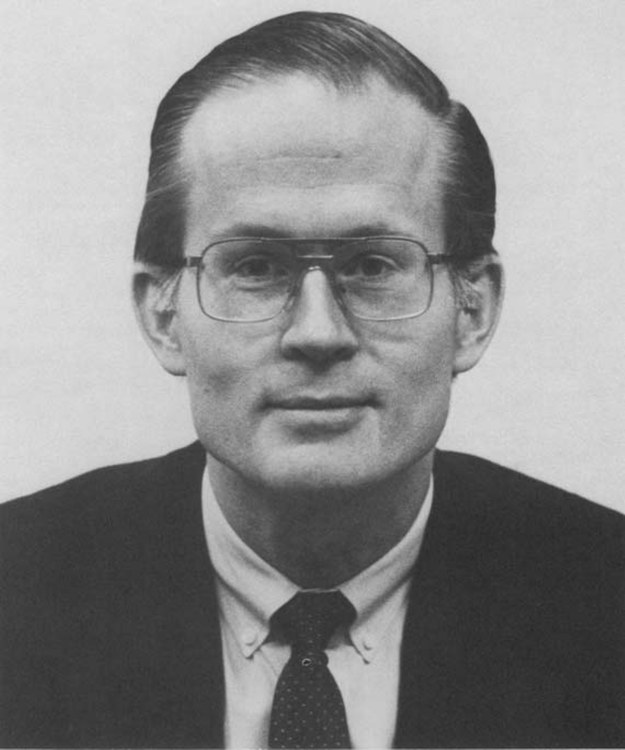
\includegraphics[height=3.9cm]{Figures/black.jpg}
		\caption*{\small Fischer Black (1938--1995)}
	\end{subfigure}\hfill
	\begin{subfigure}[b]{0.31\textwidth}
		\centering
		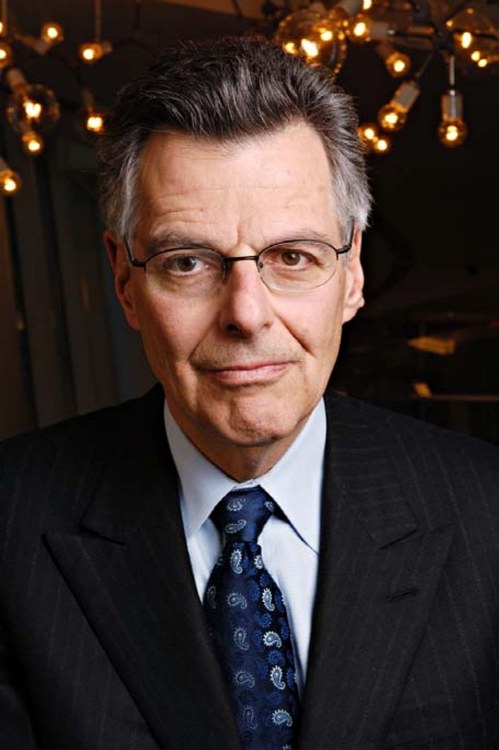
\includegraphics[height=3.9cm]{Figures/scholes.jpg}
		\caption*{\small Myron Scholes (1941--)}
	\end{subfigure}\hfill
	\begin{subfigure}[b]{0.31\textwidth}
		\centering
		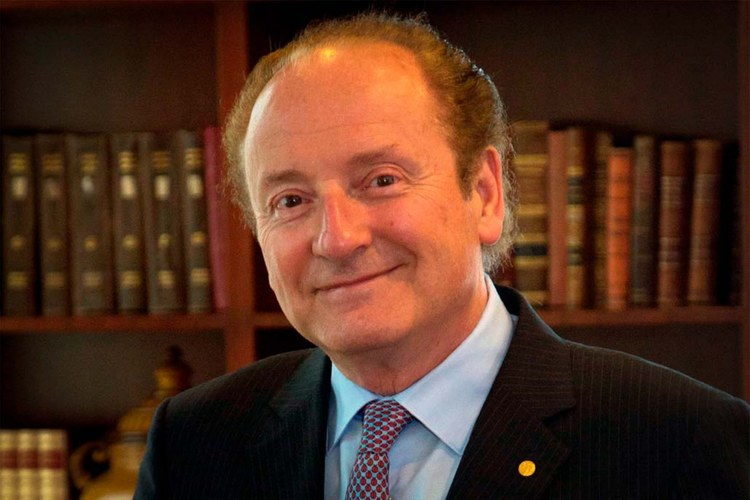
\includegraphics[height=3.9cm]{Figures/merton.jpg}
		\caption*{\small Robert C. Merton (1944--)}
	\end{subfigure}
	\caption{The authors of the 1973 breakthrough. Black had died by 1997 and
		so could not share the Nobel Prize awarded to Scholes and Merton.}
	\label{fig:bsm-portraits}
\end{figure}

\source{Slides p.~246}

\begin{notation}
	The symbols $C$, $P$, $X$ and $S$ keep the meanings fixed in \autoref{sec:payoff}.
	Two are new:
	\begin{itemize}[nosep]
		\item $\hat{r}>0$: the continuously compounded riskless rate \emph{per period};
		\item $R\triangleq e^{\hat{r}}$: the \vocab{gross return} over one period.
	\end{itemize}
	A dollar lent today is thus worth $R$ dollars one period later.
	We start from the discrete-time binomial model.
\end{notation}

%─────§ BOPM────────────────────────────────────────────────────────────────────────────────────────────────────────────────────────────────────────
\section{The Binomial Option Pricing Model}
\label{sec:bopm}

\source{Slides pp.~247--248}

\begin{definition}
	In the \vocab{binomial option pricing model} (BOPM), time is discrete and measured in periods.
	If the current stock price is $S$, one period later it is either
	\[
		Su \quad\text{with probability } q,
		\qquad\text{or}\qquad
		Sd \quad\text{with probability } 1-q ,
	\]
	where $0<q<1$ and $d<u$.
\end{definition}

In fact $d\le R\le u$ must hold to rule out arbitrage.\footnote{See Exercise 9.2.1 of the textbook. The sufficient condition is the strict one, $d<R<u$ (Björk, 2009), which we shall assume.}

\begin{intuition}
	If $R<d$ the stock beats the bond in \emph{every} state: borrow, buy stock, and collect a riskless profit.
	If $R>u$ the reverse trade does it.
	So $d<R<u$ is not a modelling convenience --- it is precisely the condition that \autoref{sec:arbitrage} is not violated by the model itself.
\end{intuition}

\begin{figure}[H]
	\centering
	\begin{tikzpicture}[font=\small, >={Stealth[length=4pt]}]
		\node (s)  at (0,0)      {$S$};
		\node (su) at (3.1,1.05) {$Su$};
		\node (sd) at (3.1,-1.05){$Sd$};
		\draw[->, MidnightBlue!75!black] (s) -- (su)
		node[midway, above left=-3pt, font=\footnotesize] {$q$};
		\draw[->, RawSienna] (s) -- (sd)
		node[midway, below left=-3pt, font=\footnotesize] {$1-q$};
	\end{tikzpicture}
	\caption{One period of the binomial model. Only the two \emph{multipliers}
		$u$ and $d$ matter; the current price $S$ scales out.}
	\label{fig:binomial-one-step}
\end{figure}

\begin{moral}
	Six pieces of information suffice to determine the option value on arbitrage considerations alone:
	\[
		S,\quad u,\quad d,\quad X,\quad \hat{r},\quad\text{and the number of periods to expiration.}
	\]
	Conspicuously absent is $q$ --- the probability that the stock goes up. \autoref{sec:bopm-risk} explains why.
\end{moral}

%─────§ Single-period call───────────────────────────────────────────────────────────────────────────────────────────────────────────────────────────
\section{A Call over a Single Period}
\label{sec:bopm-one-period}

\source{Slides pp.~249--253}

Take the expiration date to be only one period from now, and write $C_{u}$ and $C_{d}$ for the call price at time~1 after an up and a down move.
Since time~1 \emph{is} expiration, \eqref{eq:call-payoff} gives them at once:
\begin{equation}
	\begin{aligned}
		C_{u} & \;=\; \max(0,\,Su-X) , \\
		C_{d} & \;=\; \max(0,\,Sd-X) .
	\end{aligned}
	\label{eq:bopm-terminal}
\end{equation}

\begin{figure}[H]
	\centering
	\begin{tikzpicture}[font=\small, >={Stealth[length=4pt]}]
		\node (c)  at (0,0)      {$C$};
		\node (cu) at (3.1,1.05) {$C_{u}=\max(0,\,Su-X)$};
		\node (cd) at (3.1,-1.05){$C_{d}=\max(0,\,Sd-X)$};
		\draw[->, MidnightBlue!75!black] (c) -- (cu)
		node[midway, above left=-3pt, font=\footnotesize] {$q$};
		\draw[->, RawSienna] (c) -- (cd)
		node[midway, below left=-3pt, font=\footnotesize] {$1-q$};
	\end{tikzpicture}
	\caption{The call written on \autoref{fig:binomial-one-step}. The two
		terminal values are known; the problem is the value $C$ at the root.}
	\label{fig:binomial-call-one-step}
\end{figure}

The trick is to build something with the same two terminal values out of instruments whose prices we already know.

\begin{definition}
	Set up a portfolio of $h$ shares of stock and $B$ dollars in riskless bonds.
	It costs $hS+B$ today, and $h$ is called the \vocab{hedge ratio} or \vocab{delta}.
\end{definition}

The value of this portfolio at time one is
\[
	\begin{cases}
		hSu+RB, & \text{up move},  \\
		hSd+RB, & \text{down move},
	\end{cases}
\]
so choosing $h$ and $B$ to replicate the payoff of the call means solving
\begin{equation}
	\begin{aligned}
		hSu+RB & \;=\; C_{u} , \\
		hSd+RB & \;=\; C_{d} .
	\end{aligned}
	\label{eq:bopm-replicate}
\end{equation}

Two linear equations in two unknowns, with a nonsingular matrix because $u\ne d$:
\begin{equation}
	h \;=\; \frac{C_{u}-C_{d}}{Su-Sd} \;\ge\; 0 ,
	\qquad
	B \;=\; \frac{uC_{d}-dC_{u}}{(u-d)\,R} .
	\label{eq:bopm-hb}
\end{equation}

\begin{theorem}
	\label{thm:bopm-call}
	By the no-arbitrage principle, the European call must cost the same as the equivalent portfolio:\footnote{Also called the \vocab{replicating portfolio}, since it replicates the option.}
	\begin{equation}
		C \;=\; hS+B .
		\label{eq:bopm-price}
	\end{equation}
\end{theorem}

\begin{proof}
	By construction the portfolio and the call have identical payoffs in both states at time~1, so \autoref{cor:same-payoff} forces identical prices at time~0.
\end{proof}

\begin{note}
	Read off the signs. $h\ge 0$: the replicating portfolio is \emph{long} stock, as one would expect of a call. And since $uC_{d}-dC_{u}<0$ we have $B<0$, so the equivalent portfolio is a \textbf{levered long position in stocks} --- buy $h$ shares, borrow $\abs{B}$ to help pay for them.

	This also explains an option's reputation for leverage: it packages exactly that trade, and its percentage swings are correspondingly larger than the stock's.
\end{note}

\subsection{American Calls and Puts over One Period}
\label{sec:american-one-period}

\source{Slides pp.~254--255}

For an American call we have to consider immediate exercise, so
\[
	C \;=\; \max\bigl(hS+B,\; S-X\bigr) .
\]
When $hS+B\ge S-X$ the call should not be exercised immediately; when $hS+B<S-X$ it should.
For non-dividend-paying stocks the first case always holds, by \autoref{thm:merton-no-early}, so once again $C=hS+B$.

Puts are priced the same way.
Their delta is
\[
	h \;=\; \frac{P_{u}-P_{d}}{Su-Sd} \;\le\; 0 ,
	\qquad
	P_{u} = \max(0,\,X-Su) , \quad P_{d} = \max(0,\,X-Sd) ,
\]
and with $B=(uP_{d}-dP_{u})/\bigl((u-d)R\bigr)$ the European put is worth $hS+B$, while the American put is worth
\[
	\max\bigl(hS+B,\; X-S\bigr) .
\]

\begin{note}
	The $\max$ cannot be dropped this time: early exercise \emph{can} be optimal with American puts, exactly as \autoref{sec:early-exercise} warned.
	Note also that $h\le 0$ --- replicating a put means \emph{shorting} stock and lending, the mirror image of the call.
\end{note}

%─────§ Risk────────────────────────────────────────────────────────────────────────────────────────────────────────────────────────────────────────
\section{Where Did the Risk Go?}
\label{sec:bopm-risk}

\source{Slides p.~256}

Look again at \eqref{eq:bopm-hb} and \eqref{eq:bopm-price}.
Surprisingly, the option value is independent of $q$.\footnote{More precisely, not \emph{directly} dependent on $q$. Thanks to a lively class discussion on March 16, 2011.}
Hence it is also independent of the stock's expected value,
\[
	qSu+(1-q)\,Sd .
\]

The option value depends instead on the \emph{sizes} of the price changes, $u$ and $d$, which the investors must agree upon.
Given those, the set of possible stock prices is the same whatever $q$ is.

\begin{moral}
	Two investors who violently disagree about whether the stock will rise must nevertheless quote the \emph{same} option price, provided they agree on how far it can move.

	The reason is \eqref{eq:bopm-replicate}: the replicating portfolio matches the call in \emph{every} state, so how likely the states are never enters.
	This is what dissolves the risk-adjusted discount rate problem of \autoref{sec:pricing-setting} --- there is no expectation to discount, only a portfolio to price.
\end{moral}

%─────§ Pseudo probability───────────────────────────────────────────────────────────────────────────────────────────────────────────────────────────
\section{Pseudo Probability}
\label{sec:pseudo-prob}

\source{Slides pp.~257--258}

The formula $C=hS+B$ is correct but opaque.
Substituting \eqref{eq:bopm-hb} and rearranging gives
\[
	hS+B \;=\; \frac{\dfrac{R-d}{u-d}\,C_{u} + \dfrac{u-R}{u-d}\,C_{d}}{R} ,
\]
whose two coefficients are nonnegative and sum to $1$.
Naming the first of them,
\begin{equation}
	p \;\triangleq\; \frac{R-d}{u-d} ,
	\label{eq:risk-neutral-p}
\end{equation}
turns the expression into
\begin{equation}
	hS+B \;=\; \frac{p\,C_{u}+(1-p)\,C_{d}}{R} .
	\label{eq:bopm-expectation}
\end{equation}

Since $d<R<u$ we have $0<p<1$, so $p$ may be interpreted as a probability.

\begin{note}
	The interpretation is optional.
	Read without it, the numerator of \eqref{eq:bopm-expectation} simply \emph{interpolates}: the line through the points $(Su,C_{u})$ and $(Sd,C_{d})$, evaluated at $SR$, has height
	\[
		\frac{R-d}{u-d}\,C_{u} + \frac{u-R}{u-d}\,C_{d} .
	\]
	So \eqref{eq:bopm-expectation} says the option is worth the linear interpolation of its payoffs at the stock's \emph{forward} price, discounted back.
	Nothing probabilistic has happened yet --- which is precisely why the next step is legitimate.
\end{note}

%─────§ Risk-neutral probability─────────────────────────────────────────────────────────────────────────────────────────────────────────────────────
\section{The Risk-Neutral Probability}
\label{sec:risk-neutral-prob}

\source{Slides p.~259}

The quantity $p$ earns its name from one calculation.
Under $p$, the expected rate of return of the stock is exactly the riskless rate:
\begin{equation}
	p\,Su+(1-p)\,Sd \;=\; RS .
	\label{eq:rn-stock}
\end{equation}
Substituting \eqref{eq:risk-neutral-p} verifies it in one line.

Now, the expected rates of return of \emph{all} securities must equal the riskless rate when investors are risk-neutral --- a risk-neutral investor demands no compensation for bearing risk.
Equation \eqref{eq:rn-stock} says the stock behaves that way under $p$, and for this reason $p$ is called the \vocab{risk-neutral probability}.

\begin{moral}
	The value of an option is the expectation of its discounted future payoff \emph{in a risk-neutral economy}.
	So the rate used for discounting is the riskless rate --- and the obstacle raised in \autoref{sec:pricing-setting} is gone, not by being solved but by being made irrelevant.

	The risk-neutral economy is a computational fiction. Real investors are not risk-neutral, and $p\ne q$ in general.
	What \eqref{eq:bopm-expectation} asserts is only that the \emph{answer} is the same as if they were, because the replicating portfolio does not care either way.

	This is also the $f$ of \autoref{thm:breeden-litzenberger}: the density the market prices with, now constructed rather than merely observed.
\end{moral}

%─────§ Multi-period────────────────────────────────────────────────────────────────────────────────────────────────────────────────────────────────
\section{The Multi-Period Model}
\label{sec:bopm-multi}

\source{Slides pp.~260--265}

Consider a call with two periods remaining before expiration.
Under the binomial model the stock can take on three possible prices at time two: $Suu$, $Sud$ and $Sdd$.
There are four \emph{paths} --- $uu$, $ud$, $du$, $dd$ --- but the tree \vocab{recombines}, since $ud=du$, so there are only three terminal prices.

At any node the next two stock prices depend only on the current price, not on the prices of earlier times; the model is \vocab{Markovian}.

\begin{figure}[H]
	\centering
	\begin{tikzpicture}[font=\small, >={Stealth[length=4pt]},
			every node/.style={inner sep=1.5pt},
			up/.style={->, MidnightBlue!75!black},
			dn/.style={->, RawSienna}]
		\begin{scope}
			\node (s)   at (0,0)      {$S$};
			\node (su)  at (2.1,1.0)  {$Su$};
			\node (sd)  at (2.1,-1.0) {$Sd$};
			\node (suu) at (4.3,2.0)  {$Suu$};
			\node (sud) at (4.3,0)    {$Sud$};
			\node (sdd) at (4.3,-2.0) {$Sdd$};
			\draw[up] (s) -- (su);   \draw[dn] (s) -- (sd);
			\draw[up] (su) -- (suu); \draw[dn] (su) -- (sud);
			\draw[up] (sd) -- (sud); \draw[dn] (sd) -- (sdd);
		\end{scope}
		\begin{scope}[xshift=6.7cm]
			\node (c)   at (0,0)      {$C$};
			\node (cu)  at (2.1,1.0)  {$C_{u}$};
			\node (cd)  at (2.1,-1.0) {$C_{d}$};
			\node (cuu) at (4.3,2.0)  {$C_{uu}$};
			\node (cud) at (4.3,0)    {$C_{ud}$};
			\node (cdd) at (4.3,-2.0) {$C_{dd}$};
			\draw[up] (c) -- (cu);   \draw[dn] (c) -- (cd);
			\draw[up] (cu) -- (cuu); \draw[dn] (cu) -- (cud);
			\draw[up] (cd) -- (cud); \draw[dn] (cd) -- (cdd);
		\end{scope}
	\end{tikzpicture}
	\caption{Two periods. Four paths but three terminal states, because the
		tree recombines. The call tree on the right has exactly the same shape;
		only the numbers in the nodes differ.}
	\label{fig:binomial-two-step}
\end{figure}

At expiration the call's values are read off \eqref{eq:call-payoff} as before:
\[
	C_{uu} = \max(0,\,Suu-X) , \qquad
	C_{ud} = \max(0,\,Sud-X) , \qquad
	C_{dd} = \max(0,\,Sdd-X) .
\]

The call values at time~1 are then obtained by applying \eqref{eq:bopm-expectation} to each node:
\begin{equation}
	C_{u} \;=\; \frac{p\,C_{uu}+(1-p)\,C_{ud}}{R} ,
	\qquad
	C_{d} \;=\; \frac{p\,C_{ud}+(1-p)\,C_{dd}}{R} .
	\label{eq:bopm-step-back}
\end{equation}
Deltas come from \eqref{eq:bopm-hb}; for example the delta at $C_{u}$ is $(C_{uu}-C_{ud})/(Suu-Sud)$.

We now reach the current period and compute
\[
	C \;=\; \frac{p\,C_{u}+(1-p)\,C_{d}}{R} ,
\]
with $h$ and $B$ again from \eqref{eq:bopm-hb}.

\subsection{Early Exercise, Again}

\source{Slides p.~266}

The tree lets us re-derive \autoref{thm:merton-no-early} by direct computation.
Since the call will not be exercised at time~1 even if it is American, $C_{u}\ge Su-X$ and $C_{d}\ge Sd-X$.
Therefore
\[
	hS+B \;=\; \frac{p\,C_{u}+(1-p)\,C_{d}}{R}
	\;\ge\; \frac{\bigl[\,pu+(1-p)\,d\,\bigr]S-X}{R}
	\;=\; S-\frac{X}{R}
	\;>\; S-X ,
\]
using \eqref{eq:rn-stock} for the middle equality and $R>1$ for the last.
So the call will not be exercised at present either, and
\[
	C \;=\; hS+B \;=\; \frac{p\,C_{u}+(1-p)\,C_{d}}{R} .
\]

%─────§ Backward induction───────────────────────────────────────────────────────────────────────────────────────────────────────────────────────────
\section{Backward Induction}
\label{sec:backward-induction}

\source{Slides pp.~267--268}

The expression above calculates $C$ from the two successor nodes $C_{u}$ and $C_{d}$ and none beyond; and the same computation happened at $C_{u}$ and $C_{d}$ themselves, in \eqref{eq:bopm-step-back}.
This recursive procedure is called \vocab{backward induction}.\footnote{Ernst Zermelo (1871--1953).}

Unrolling it for two periods,
\begin{equation}
	\begin{aligned}
		C & \;=\; \Bigl[\,p^{2}C_{uu}+2p(1-p)\,C_{ud}+(1-p)^{2}C_{dd}\,\Bigr]\Big/R^{2}                        \\
		  & \;=\; \Bigl[\,p^{2}\max\bigl(0,Su^{2}-X\bigr)+2p(1-p)\max\bigl(0,Sud-X\bigr)                       \\
		  & \hphantom{\;=\;\Bigl[\,}+\,(1-p)^{2}\max\bigl(0,Sd^{2}-X\bigr)\Bigr]\Big/R^{2} .
	\end{aligned}
	\label{eq:bopm-two-period}
\end{equation}

The coefficient $2$ on the middle term is the number of paths reaching that state, and it is the only trace the paths leave.

\begin{figure}[H]
	\centering
	\begin{tikzpicture}[font=\small, >={Stealth[length=4pt]},
			every node/.style={inner sep=1.5pt},
			up/.style={->, MidnightBlue!75!black},
			dn/.style={->, RawSienna}]
		\node (s)   at (0,0)      {$S_{0}$};
		\node (su)  at (2.4,1.1)  {$S_{0}u$};
		\node (sd)  at (2.4,-1.1) {$S_{0}d$};
		\node (suu) at (5.0,2.2)  {$S_{0}u^{2}$};
		\node (sud) at (5.0,0)    {$S_{0}ud$};
		\node (sdd) at (5.0,-2.2) {$S_{0}d^{2}$};
		\draw[up] (s) -- (su) node[midway, above left=-3pt, font=\footnotesize] {$p$};
		\draw[dn] (s) -- (sd) node[midway, below left=-3pt, font=\footnotesize] {$1-p$};
		\draw[up] (su) -- (suu); \draw[dn] (su) -- (sud);
		\draw[up] (sd) -- (sud); \draw[dn] (sd) -- (sdd);
		\node[anchor=west, font=\footnotesize, text=Gray!45!black]
		at (6.1,2.2) {$p^{2}$};
		\node[anchor=west, font=\footnotesize, text=Gray!45!black]
		at (6.1,0) {$2p(1-p)$};
		\node[anchor=west, font=\footnotesize, text=Gray!45!black]
		at (6.1,-2.2) {$(1-p)^{2}$};
	\end{tikzpicture}
	\caption{The two-period tree with risk-neutral probabilities. The terminal
		weights in \eqref{eq:bopm-two-period} are the binomial probabilities
		$\binom{2}{j}p^{j}(1-p)^{2-j}$.}
	\label{fig:binomial-probs}
\end{figure}

\source{Slides p.~269}

In the $n$-period case the same unrolling gives
\begin{equation}
	C \;=\; \frac{\displaystyle\sum_{j=0}^{n}\binom{n}{j}p^{j}(1-p)^{n-j}\times\max\bigl(0,\,Su^{j}d^{n-j}-X\bigr)}{R^{n}} ,
	\label{eq:bopm-call-n}
\end{equation}
and similarly for the put,
\begin{equation}
	P \;=\; \frac{\displaystyle\sum_{j=0}^{n}\binom{n}{j}p^{j}(1-p)^{n-j}\times\max\bigl(0,\,X-Su^{j}d^{n-j}\bigr)}{R^{n}} .
	\label{eq:bopm-put-n}
\end{equation}

\begin{moral}
	The value of a call on a non-dividend-paying stock is the expected discounted payoff at expiration in a risk-neutral economy --- literally the sum in \eqref{eq:bopm-call-n}, with $\binom{n}{j}p^{j}(1-p)^{n-j}$ as the probability of finishing in state $j$.

	Note what \eqref{eq:bopm-call-n} is \emph{not}: it is not a shortcut that skips the tree. It is the tree, summed. For a European option the two agree; for an American one only the tree works, because the $\max$ against intrinsic value has to be taken at every node.
\end{moral}

\subsection{Reading the Weights as State Prices}

\source{Slides p.~270}

Define
\begin{equation}
	p_{j} \;\triangleq\; \frac{\binom{n}{j}p^{j}(1-p)^{n-j}}{R^{n}} ,
	\qquad j=0,1,\ldots,n .
	\label{eq:bopm-state-price}
\end{equation}
This is the \emph{state price} of \autoref{sec:state-price-density}, now for the state $Su^{j}d^{n-j}$: the price today of a claim paying \$1 there and nothing elsewhere.
In general, then,
\[
	\text{option price} \;=\; \sum_{j}\bigl(p_{j}\times\text{payoff at state } j\bigr) ,
\]
and \eqref{eq:bopm-call-n} and \eqref{eq:bopm-put-n} are two instances of it.

\begin{note}
	The butterfly construction of \autoref{sec:state-price-density} works here literally, and the discrete states simplify it.\footnote{Bahra (1997).}
	Buy $(X_{M}-X_{L})^{-1}$ units of the butterfly spread with
	\[
		X_{L}=Su^{j-1}d^{n-j+1} , \qquad
		X_{M}=Su^{j}d^{n-j} , \qquad
		X_{H}=Su^{j+1}d^{n-j-1} ,
	\]
	that is, struck at the state itself and its two neighbours.
	No stock price strictly between $X_{L}$ and $X_{H}$ is attainable except $X_{M}$, so the tent's \emph{whole} payoff is the single value $1$ at state $j$; the exponent $-1$ replaces the $-2$ of the continuous case, where the tent had to be scaled by area instead.
	Its price is therefore $p_{j}$, and $R^{n}p_{j}=\binom{n}{j}p^{j}(1-p)^{n-j}$ is the undiscounted state price --- the risk-neutral probability.
\end{note}

%─────§ Risk-neutral pricing methodology─────────────────────────────────────────────────────────────────────────────────────────────────────────────
\section{The Risk-Neutral Pricing Methodology}
\label{sec:rn-methodology}

\source{Slides p.~271}

Nothing in the argument used the payoff $\max(0,S-X)$ beyond the fact that it was a function of the terminal stock price.
So the conclusion generalises at once.

\begin{moral}
	Every derivative can be priced as if the economy were risk-neutral.
	For a European-style derivative with terminal payoff function $D$, its value is
	\begin{equation}
		e^{-\hat{r}n}\,E^{\pi}[\,D\,] ,
		\label{eq:rn-pricing}
	\end{equation}
	where $E^{\pi}$ means the expectation is taken under the risk-neutral probability.
\end{moral}

The ``equivalence'' between arbitrage freedom in a model and the existence of a risk-neutral probability is called the \vocab{(first) fundamental theorem of asset pricing}.\footnote{Dybvig \& Ross (1987).}

\begin{figure}[H]
	\centering
	\begin{subfigure}[b]{0.34\textwidth}
		\centering
		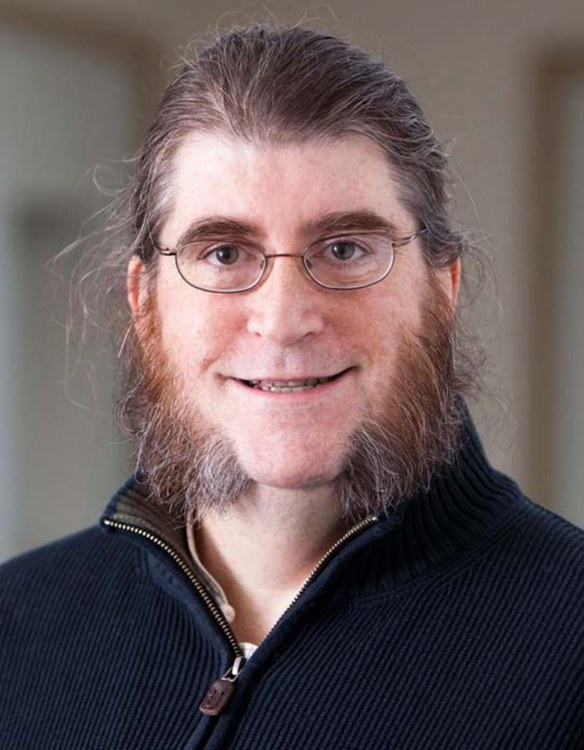
\includegraphics[height=3.9cm]{Figures/dybvig.jpg}
		\caption*{\small Philip H. Dybvig (1955--)}
	\end{subfigure}\hspace{0.05\textwidth}
	\begin{subfigure}[b]{0.34\textwidth}
		\centering
		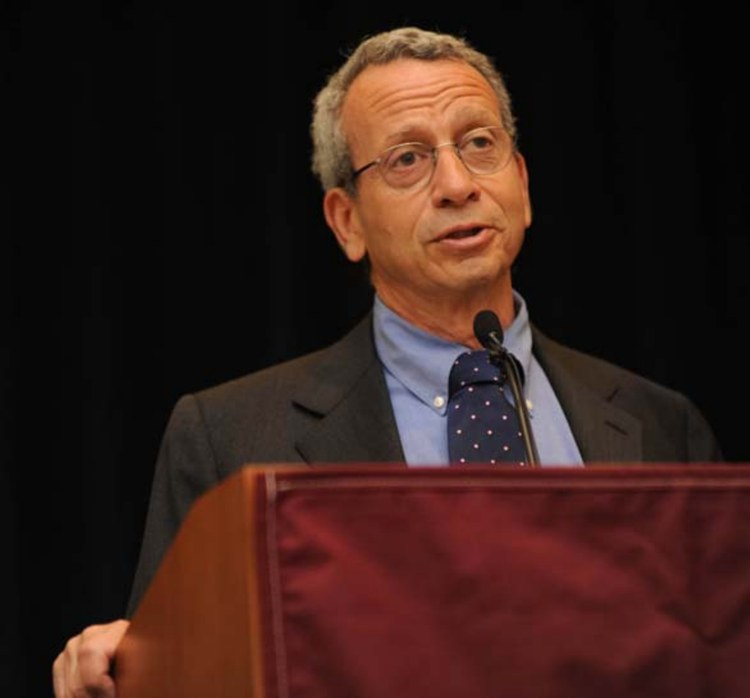
\includegraphics[height=3.9cm]{Figures/ross.jpg}
		\caption*{\small Stephen Ross (1944--2017)}
	\end{subfigure}
	\caption{Dybvig, co-winner of the 2022 Nobel Prize in Economic Sciences,
		and Ross --- whose 1976 replication theorem already appeared as
		\autoref{thm:piecewise-replication}.}
	\label{fig:dybvig-ross}
\end{figure}

\begin{note}
	The theorem closes the circle this course opened with.
	Chapter~\ref{ch:arbitrage} assumed no arbitrage and extracted relations between prices; \autoref{sec:risk-neutral-prob} built a probability $\pi$ out of a particular model.
	The fundamental theorem says these are two descriptions of the same thing: a model admits no arbitrage \emph{exactly} when such a $\pi$ exists.
	Pricing a derivative and checking a model for consistency are therefore one problem.
\end{note}

%─────§ Self-financing───────────────────────────────────────────────────────────────────────────────────────────────────────────────────────────────
\section{Self-Financing}
\label{sec:self-financing}

\source{Slides p.~274}

One loose end remains.
The delta $h$ of \eqref{eq:bopm-hb} is computed node by node, and it changes as the stock moves, so the maintenance of an equivalent portfolio is \emph{dynamic}: the replicating position must be rebalanced every period.

That sounds expensive, and it raises the obvious worry --- if rebalancing requires fresh money, the option's price is not really $hS+B$.
It does not.

\begin{proposition}
	\label{prop:self-financing}
	The replicating strategy is \vocab{self-financing}: there is neither injection nor withdrawal of funds throughout.\footnote{Except at the beginning, of course, when the option premium is paid before the replication starts.}
\end{proposition}

The reason is already in \eqref{eq:bopm-replicate}.
At the end of the current period the portfolio is worth $hSu+RB$ or $hSd+RB$, which \emph{is} $C_{u}$ or $C_{d}$ --- and $C_{u}$ and $C_{d}$ are, by \eqref{eq:bopm-price} applied one period later, exactly the cost of the next portfolio.
The portfolio's value at the end of each period is therefore precisely the amount needed to set up the next one.
Changes in value are due entirely to capital gains.

\begin{moral}
	Rebalancing does not depend on predicting future stock prices.

	The delta at each node is a function of where the stock \emph{is}, not of where it is going; the strategy is told what to do by the tree, and it always has exactly enough money to do it.
	That is the whole content of ``the option is worth its replicating portfolio'', and it is what makes \eqref{eq:rn-pricing} a hedging recipe rather than merely a formula.
\end{moral}
